\setcounter{definition}{0} \setcounter{property}{0} \setcounter{claim}{0} \setcounter{fact}{0} \setcounter{corollary}{0} \setcounter{figure}{0}
\section{Maximum Flow and Minimum Cut}


A \emph{network}~(also called \emph{flow network}) models 
an abstracted flow~(traffic, data, etc) transmits from an origin to a destination
via a graphical structure. Formally, a (flow) network is a tuple $(G = (V, E), s, t, c(\cdot))$, where
%$G = (V, E)$ is a directed graph, $s\in V$ represents the source vertex~(i.e., the in-degree of $s$ is 0),
%$t\in V$ represents the sink vertex~(i.e., the out-degree of $t$ is 0),
%and $c(e) \ge 0$ represents the \emph{capacity} of edge $e\in E$.

\vspace*{-\topsep}
\begin{enumerate}
\item $G = (V, E)$ is a directed graph;
\item $s\in V$ is a source vertex of $G$~(i.e., the in-degree of $s$ is 0), from which the flow is generated;
\item $t\in V$ is a sink vertex of $G$~(i.e., the out-degree of $t$ is 0), at which the flow is absorbed;
\item $c: E\to \mathbb{R}^+$, in which $c(e)$ represents the \emph{capacity} of edge $e\in E$, which models the limit of the flow that edge $e$ can carry.
\end{enumerate}

An \emph{$s$-$t$ flow} of network $(G = (V, E), s, t, c(\cdot))$
describes {how} the flow is transmitted from $s$ to $t$
via the graph $G$ under the capacity constraints. Formally,
an $s$-$t$ flow $f$ is a function $f: E\to \mathbb{R}_{\ge 0}$
that satisfies the following two conditions:
\vspace*{-\topsep}
\begin{enumerate}
\item For every $e\in E$, $0\le f(e) \le c(e)$; this is called the \emph{capacity condition};
\item For every vertex $v\in V\setminus\{s,t\}$, $\sum_{e\in I(v)} f(e) = \sum_{e\in O(v)} f(e)$, where $I(v) := \{(u,v)\in E\mid u\in V\}$ represents
the set of in-edges of $v$, and $O(v) := \{(v,w)\in E\mid w\in V\}$ represents
the set of out-edges of $v$. This is called the \emph{conservation condition}.
\end{enumerate}

Intuitively, an $s$-$t$ flow assigns an non-negative value $f(e)$ to edge $e$, representing the
amount of flow that is carried by edge $e$; such amount must not exceed the capacity of $e$, i.e., $f(e) \le c(e)$, for every $e\in E$.
All vertices, except the source $s$ that generates the flow and the sink that absorbs the flow,
redistribute the flow~(instead of repositing any flow); therefore, for each vertex $v\in V\setminus\{s,t\}$,
the total amount of flow that enters $v$ equals to the total amount of flow that leaves $v$.
See Figure~\ref{fig:flow}.

\begin{figure}[h]
\centering{

\tikzset{every picture/.style={line width=0.75pt}} %set default line width to 0.75pt        

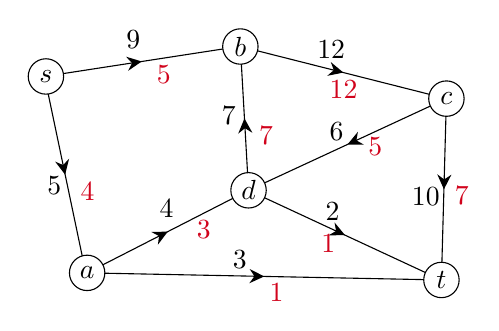
\begin{tikzpicture}[x=0.5pt,y=0.5pt,yscale=-1,xscale=1]
%uncomment if require: \path (0,222); %set diagram left start at 0, and has height of 222

%Straight Lines [id:da3853598268579197] 
\draw    (24.79,46.83) -- (165.31,25.18) ;
\draw [shift={(95.05,36)}, rotate = 531.24] [fill={rgb, 255:red, 0; green, 0; blue, 0 }  ][line width=0.08]  [draw opacity=0] (10.72,-5.15) -- (0,0) -- (10.72,5.15) -- (7.12,0) -- cycle    ;
%Straight Lines [id:da6958538828947681] 
\draw    (24.79,46.83) -- (54.58,188.77) ;
\draw [shift={(39.69,117.8)}, rotate = 258.15] [fill={rgb, 255:red, 0; green, 0; blue, 0 }  ][line width=0.08]  [draw opacity=0] (10.72,-5.15) -- (0,0) -- (10.72,5.15) -- (7.12,0) -- cycle    ;
%Straight Lines [id:da2980592918523626] 
\draw    (55.58,188.77) -- (311.62,193.9) ;
\draw [shift={(183.6,191.34)}, rotate = 181.15] [fill={rgb, 255:red, 0; green, 0; blue, 0 }  ][line width=0.08]  [draw opacity=0] (10.72,-5.15) -- (0,0) -- (10.72,5.15) -- (7.12,0) -- cycle    ;
%Straight Lines [id:da14604600957867897] 
\draw    (172.22,129.11) -- (311.62,193.9) ;
\draw [shift={(241.92,161.5)}, rotate = 204.92000000000002] [fill={rgb, 255:red, 0; green, 0; blue, 0 }  ][line width=0.08]  [draw opacity=0] (10.72,-5.15) -- (0,0) -- (10.72,5.15) -- (7.12,0) -- cycle    ;
%Straight Lines [id:da8640956582518242] 
\draw    (166.31,25.18) -- (172.22,129.11) ;
\draw [shift={(169.27,77.14)}, rotate = 86.75] [fill={rgb, 255:red, 0; green, 0; blue, 0 }  ][line width=0.08]  [draw opacity=0] (10.72,-5.15) -- (0,0) -- (10.72,5.15) -- (7.12,0) -- cycle    ;
%Straight Lines [id:da285469110869773] 
\draw    (166.31,25.18) -- (315.22,62.84) ;
\draw [shift={(240.76,44.01)}, rotate = 194.2] [fill={rgb, 255:red, 0; green, 0; blue, 0 }  ][line width=0.08]  [draw opacity=0] (10.72,-5.15) -- (0,0) -- (10.72,5.15) -- (7.12,0) -- cycle    ;
%Straight Lines [id:da8162300663234149] 
\draw    (315.22,62.84) -- (311.62,193.9) ;
\draw [shift={(313.42,128.37)}, rotate = 271.57] [fill={rgb, 255:red, 0; green, 0; blue, 0 }  ][line width=0.08]  [draw opacity=0] (10.72,-5.15) -- (0,0) -- (10.72,5.15) -- (7.12,0) -- cycle    ;
%Straight Lines [id:da5085854502811855] 
\draw    (315.22,62.84) -- (172.22,129.11) ;
\draw [shift={(243.72,95.98)}, rotate = 335.13] [fill={rgb, 255:red, 0; green, 0; blue, 0 }  ][line width=0.08]  [draw opacity=0] (10.72,-5.15) -- (0,0) -- (10.72,5.15) -- (7.12,0) -- cycle    ;
%Straight Lines [id:da4064365628912957] 
\draw    (172.22,129.11) -- (55.58,188.77) ;
\draw [shift={(113.9,158.94)}, rotate = 152.91] [fill={rgb, 255:red, 0; green, 0; blue, 0 }  ][line width=0.08]  [draw opacity=0] (10.72,-5.15) -- (0,0) -- (10.72,5.15) -- (7.12,0) -- cycle    ;
%Shape: Ellipse [id:dp651117123053256] 
\draw  [fill={rgb, 255:red, 255; green, 255; blue, 255 }  ,fill opacity=1 ] (13,46.83) .. controls (13,39.77) and (18.73,34.04) .. (25.79,34.04) .. controls (32.86,34.04) and (38.58,39.77) .. (38.58,46.83) .. controls (38.58,53.9) and (32.86,59.62) .. (25.79,59.62) .. controls (18.73,59.62) and (13,53.9) .. (13,46.83) -- cycle ;
%Shape: Ellipse [id:dp7399561756845123] 
\draw  [fill={rgb, 255:red, 255; green, 255; blue, 255 }  ,fill opacity=1 ] (153.52,25.18) .. controls (153.52,18.11) and (159.25,12.39) .. (166.31,12.39) .. controls (173.38,12.39) and (179.1,18.11) .. (179.1,25.18) .. controls (179.1,32.24) and (173.38,37.97) .. (166.31,37.97) .. controls (159.25,37.97) and (153.52,32.24) .. (153.52,25.18) -- cycle ;
%Shape: Ellipse [id:dp8268258265249401] 
\draw  [fill={rgb, 255:red, 255; green, 255; blue, 255 }  ,fill opacity=1 ] (302.43,62.84) .. controls (302.43,55.78) and (308.15,50.05) .. (315.22,50.05) .. controls (322.28,50.05) and (328.01,55.78) .. (328.01,62.84) .. controls (328.01,69.9) and (322.28,75.63) .. (315.22,75.63) .. controls (308.15,75.63) and (302.43,69.9) .. (302.43,62.84) -- cycle ;
%Shape: Ellipse [id:dp5421818862330341] 
\draw  [fill={rgb, 255:red, 255; green, 255; blue, 255 }  ,fill opacity=1 ] (159.43,129.11) .. controls (159.43,122.05) and (165.15,116.32) .. (172.22,116.32) .. controls (179.28,116.32) and (185.01,122.05) .. (185.01,129.11) .. controls (185.01,136.18) and (179.28,141.9) .. (172.22,141.9) .. controls (165.15,141.9) and (159.43,136.18) .. (159.43,129.11) -- cycle ;
%Shape: Ellipse [id:dp45600813719389455] 
\draw  [fill={rgb, 255:red, 255; green, 255; blue, 255 }  ,fill opacity=1 ] (42.79,188.77) .. controls (42.79,181.71) and (48.52,175.98) .. (55.58,175.98) .. controls (62.64,175.98) and (68.37,181.71) .. (68.37,188.77) .. controls (68.37,195.84) and (62.64,201.56) .. (55.58,201.56) .. controls (48.52,201.56) and (42.79,195.84) .. (42.79,188.77) -- cycle ;
%Shape: Ellipse [id:dp031187496945339066] 
\draw  [fill={rgb, 255:red, 255; green, 255; blue, 255 }  ,fill opacity=1 ] (298.83,193.9) .. controls (298.83,186.83) and (304.56,181.11) .. (311.62,181.11) .. controls (318.69,181.11) and (324.41,186.83) .. (324.41,193.9) .. controls (324.41,200.96) and (318.69,206.69) .. (311.62,206.69) .. controls (304.56,206.69) and (298.83,200.96) .. (298.83,193.9) -- cycle ;

% Text Node
\draw (25.79,46.83) node   [align=left] {$\displaystyle s$};
% Text Node
\draw (166.31,25.18) node   [align=left] {$\displaystyle b$};
% Text Node
\draw (315.22,62.84) node   [align=left] {$\displaystyle c$};
% Text Node
\draw (172.22,129.11) node   [align=left] {$\displaystyle d$};
% Text Node
\draw (55.58,188.77) node   [align=left] {$\displaystyle a$};
% Text Node
\draw (311.62,193.9) node   [align=left] {$\displaystyle t$};
% Text Node
\draw (229,48) node [anchor=north west][inner sep=0.75pt]   [align=left] {$\displaystyle \textcolor[rgb]{0.82,0.01,0.11}{12}$};
% Text Node
\draw (25,117) node [anchor=north west][inner sep=0.75pt]   [align=left] {$\displaystyle 5$};
% Text Node
\draw (106,134) node [anchor=north west][inner sep=0.75pt]   [align=left] {$\displaystyle 4$};
% Text Node
\draw (185.6,194.34) node [anchor=north west][inner sep=0.75pt]   [align=left] {$\displaystyle \textcolor[rgb]{0.82,0.01,0.11}{1}$};
% Text Node
\draw (82,12) node [anchor=north west][inner sep=0.75pt]   [align=left] {$\displaystyle 9$};
% Text Node
\draw (229,78) node [anchor=north west][inner sep=0.75pt]   [align=left] {$\displaystyle 6$};
% Text Node
\draw (151,67) node [anchor=north west][inner sep=0.75pt]   [align=left] {$\displaystyle 7$};
% Text Node
\draw (226,136) node [anchor=north west][inner sep=0.75pt]   [align=left] {$\displaystyle 2$};
% Text Node
\draw (319.42,124.37) node [anchor=north west][inner sep=0.75pt]   [align=left] {$\displaystyle \textcolor[rgb]{0.82,0.01,0.11}{7}$};
% Text Node
\draw (133,149) node [anchor=north west][inner sep=0.75pt]   [align=left] {$\displaystyle \textcolor[rgb]{0.82,0.01,0.11}{3}$};
% Text Node
\draw (223,159) node [anchor=north west][inner sep=0.75pt]   [align=left] {$\displaystyle \textcolor[rgb]{0.82,0.01,0.11}{1}$};
% Text Node
\draw (257,89) node [anchor=north west][inner sep=0.75pt]   [align=left] {$\displaystyle \textcolor[rgb]{0.82,0.01,0.11}{5}$};
% Text Node
\draw (178,81) node [anchor=north west][inner sep=0.75pt]   [align=left] {$\displaystyle \textcolor[rgb]{0.82,0.01,0.11}{7}$};
% Text Node
\draw (288.42,125.37) node [anchor=north west][inner sep=0.75pt]   [align=left] {$\displaystyle 10$};
% Text Node
\draw (220,19) node [anchor=north west][inner sep=0.75pt]   [align=left] {$\displaystyle 12$};
% Text Node
\draw (49,122) node [anchor=north west][inner sep=0.75pt]   [align=left] {$\displaystyle \textcolor[rgb]{0.82,0.01,0.11}{4}$};
% Text Node
\draw (104,37) node [anchor=north west][inner sep=0.75pt]   [align=left] {$\displaystyle \textcolor[rgb]{0.82,0.01,0.11}{5}$};
% Text Node
\draw (159,171) node [anchor=north west][inner sep=0.75pt]   [align=left] {$\displaystyle 3$};


\end{tikzpicture}

}
\caption{Two examples of networks and $s$-$t$ flows.
The capacities are marked as black numbers next to edges;
the flow values are marked as red numbers next to edges.
The value of the flow in the left exampe is 9;
the value of the flow in the right exampe is 7;}
\label{fig:flow}
\end{figure}

The \emph{value} of an $s$-$t$ flow $f$, denoted as $|f|$,
is defined as the total amount of flow that is generated from source vertex $s$:
$|f| := \sum_{e\in O(s)} f(e)$. Intuitively, the total amount of flow that is generated
from $s$ eventually must be fully absorbed by sink $t$, as all internal vertex~(i.e., $V\setminus\{s,t\}$)
does not keep any flow. Therefore, we must have that 
$|f| = \sum_{e\in I(t)} f(e)$.  
This property is also a direct consequence of the conservation property.
Below we formally state and prove it.

\begin{fact}
We have $\sum_{e\in O(s)} f(e) = \sum_{e\in I(t)} f(e)$. 
\end{fact}

\emph{Proof.} According to the conservation condition:
$\sum_{e\in I(v)} f(e) = \sum_{e\in O(v)} f(e)$, 
for every vertex $v\in V\setminus\{s,t\}$. 
We sum up both sides over all $v\in V\setminus\{s,t\}$: 
we have $\sum_{v\in V\setminus\{s,t\}} \sum_{e\in I(v)} f(e) = \sum_{v\in V\setminus\{s,t\}} \sum_{e\in O(v)} f(e)$. 

We now break down the left side 
$L := \sum_{v\in V\setminus\{s,t\}} \sum_{e\in I(v)} f(e) 
= \sum_{v\in V} \sum_{e\in I(v)} f(e) -  \sum_{e\in I(s)} f(e) - \sum_{e\in I(t)} f(e)$.
Notice also that $\sum_{v\in V} \sum_{e\in I(v)} f(e) = \sum_{e\in E} f(e)$.
Since $s$ is a source vertex, we have $I(s) = \emptyset$, and therefore $\sum_{e\in I(s)} f(e)  = 0$.
Hence, $L = \sum_{e\in E} f(e) - \sum_{e\in I(t)} f(e)$.

Similarly, the right side 
$R := \sum_{v\in V\setminus\{s,t\}} \sum_{e\in O(v)} f(e) 
= \sum_{v\in V} \sum_{e\in O(v)} f(e) -  \sum_{e\in O(s)} f(e) - \sum_{e\in O(t)} f(e)$.
Again we have $\sum_{v\in V} \sum_{e\in O(v)} f(e) = \sum_{e\in E} f(e)$.
Since $t$ is a sink, we have $O(t) = \emptyset$, and therefore $\sum_{e\in O(t)} f(e)  = 0$.
Hence, $R = \sum_{e\in E} f(e) - \sum_{e\in O(s)} f(e)$.

Combining $L = R$ and noticing that $\sum_{e\in E} f(e)$ is shared, we have $\sum_{e\in O(s)} f(e) = \sum_{e\in I(t)} f(e)$, as desired.  \qed

We now define the \emph{maximum-flow problem}: given network $(G= (V, E), s, t, c(\cdot))$,
to find an $s$-$t$ flow $f$ such that $|f|$ is maximized.

See Figure~\ref{fig:maxflow} for an example, which shows a flow with value 
of 9. This flow has a larger value than the flow in Figure~1~(right panel,
same network, but with a flow of value 7).
Can you play with this example to try to obtain a flow with even larger value?
Is this flow~(of value 9) the maximum flow of the network?
If it is, how can we verify it is one maximum flow?
Let's answer these questions using $s$-$t$ cut.

%Playing with the instance you may find
%a flow $f$ with $|f| = 9$, shown with red numbers in the figure.
%It seems that this flow $f$ is a maximum flow.
%Here is an argument that this flow $f$ is indeed a maximum flow.
%Consider the \emph{cut} shown with blue curve. Notice that
%$s$ and $t$ are on different sides of this cut. Therefore, all flow
%from $s$ to $t$ must cross this cut. Notice also that there are three
%cut-edges~(i.e., edges cross the border from $s$-side to $t$-side)
%and the \emph{total capacities} of these 3 edges is $3 + 2 + 4 = 9$.
%This gives an \emph{upper bound} of the maximum flow, which is 9.
%And, we have found a flow $f$ with $|f| = 9$. Therefore, $f$
%is a maximum flow.

\begin{figure}[h]
\centering{

\tikzset{every picture/.style={line width=0.75pt}} %set default line width to 0.75pt        

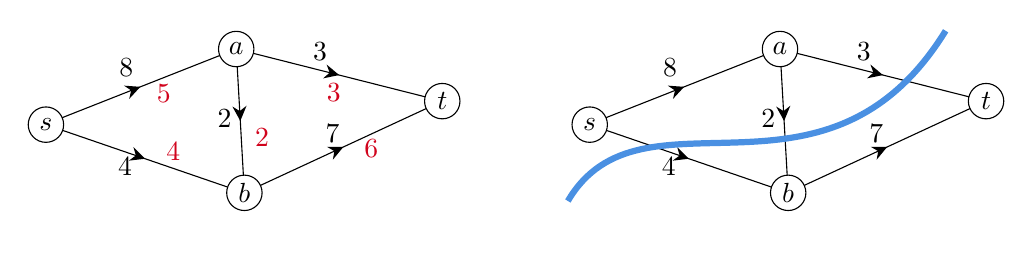
\begin{tikzpicture}[x=0.5pt,y=0.5pt,yscale=-1,xscale=1]
%uncomment if require: \path (0,166); %set diagram left start at 0, and has height of 166

%Straight Lines [id:da3853598268579197] 
\draw    (26.79,81.83) -- (165.31,27.18) ;
\draw [shift={(96.05,54.5)}, rotate = 518.47] [fill={rgb, 255:red, 0; green, 0; blue, 0 }  ][line width=0.08]  [draw opacity=0] (10.72,-5.15) -- (0,0) -- (10.72,5.15) -- (7.12,0) -- cycle    ;
%Straight Lines [id:da14604600957867897] 
\draw    (27.79,81.83) -- (171.22,131.11) ;
\draw [shift={(99.51,106.47)}, rotate = 198.96] [fill={rgb, 255:red, 0; green, 0; blue, 0 }  ][line width=0.08]  [draw opacity=0] (10.72,-5.15) -- (0,0) -- (10.72,5.15) -- (7.12,0) -- cycle    ;
%Straight Lines [id:da8640956582518242] 
\draw    (165.31,27.18) -- (171.22,131.11) ;
\draw [shift={(168.27,79.14)}, rotate = 266.75] [fill={rgb, 255:red, 0; green, 0; blue, 0 }  ][line width=0.08]  [draw opacity=0] (10.72,-5.15) -- (0,0) -- (10.72,5.15) -- (7.12,0) -- cycle    ;
%Straight Lines [id:da285469110869773] 
\draw    (165.31,27.18) -- (314.22,64.84) ;
\draw [shift={(239.76,46.01)}, rotate = 194.2] [fill={rgb, 255:red, 0; green, 0; blue, 0 }  ][line width=0.08]  [draw opacity=0] (10.72,-5.15) -- (0,0) -- (10.72,5.15) -- (7.12,0) -- cycle    ;
%Straight Lines [id:da5085854502811855] 
\draw    (314.22,64.84) -- (171.22,131.11) ;
\draw [shift={(242.72,97.98)}, rotate = 155.13] [fill={rgb, 255:red, 0; green, 0; blue, 0 }  ][line width=0.08]  [draw opacity=0] (10.72,-5.15) -- (0,0) -- (10.72,5.15) -- (7.12,0) -- cycle    ;
%Shape: Ellipse [id:dp651117123053256] 
\draw  [fill={rgb, 255:red, 255; green, 255; blue, 255 }  ,fill opacity=1 ] (15,81.83) .. controls (15,74.77) and (20.73,69.04) .. (27.79,69.04) .. controls (34.86,69.04) and (40.58,74.77) .. (40.58,81.83) .. controls (40.58,88.9) and (34.86,94.62) .. (27.79,94.62) .. controls (20.73,94.62) and (15,88.9) .. (15,81.83) -- cycle ;
%Shape: Ellipse [id:dp7399561756845123] 
\draw  [fill={rgb, 255:red, 255; green, 255; blue, 255 }  ,fill opacity=1 ] (152.52,27.18) .. controls (152.52,20.11) and (158.25,14.39) .. (165.31,14.39) .. controls (172.38,14.39) and (178.1,20.11) .. (178.1,27.18) .. controls (178.1,34.24) and (172.38,39.97) .. (165.31,39.97) .. controls (158.25,39.97) and (152.52,34.24) .. (152.52,27.18) -- cycle ;
%Shape: Ellipse [id:dp8268258265249401] 
\draw  [fill={rgb, 255:red, 255; green, 255; blue, 255 }  ,fill opacity=1 ] (301.43,64.84) .. controls (301.43,57.78) and (307.15,52.05) .. (314.22,52.05) .. controls (321.28,52.05) and (327.01,57.78) .. (327.01,64.84) .. controls (327.01,71.9) and (321.28,77.63) .. (314.22,77.63) .. controls (307.15,77.63) and (301.43,71.9) .. (301.43,64.84) -- cycle ;
%Shape: Ellipse [id:dp5421818862330341] 
\draw  [fill={rgb, 255:red, 255; green, 255; blue, 255 }  ,fill opacity=1 ] (158.43,131.11) .. controls (158.43,124.05) and (164.15,118.32) .. (171.22,118.32) .. controls (178.28,118.32) and (184.01,124.05) .. (184.01,131.11) .. controls (184.01,138.18) and (178.28,143.9) .. (171.22,143.9) .. controls (164.15,143.9) and (158.43,138.18) .. (158.43,131.11) -- cycle ;
%Straight Lines [id:da7732947748811675] 
\draw    (419.79,81.83) -- (558.31,27.18) ;
\draw [shift={(489.05,54.5)}, rotate = 518.47] [fill={rgb, 255:red, 0; green, 0; blue, 0 }  ][line width=0.08]  [draw opacity=0] (10.72,-5.15) -- (0,0) -- (10.72,5.15) -- (7.12,0) -- cycle    ;
%Straight Lines [id:da1657956393922747] 
\draw    (420.79,81.83) -- (564.22,131.11) ;
\draw [shift={(492.51,106.47)}, rotate = 198.96] [fill={rgb, 255:red, 0; green, 0; blue, 0 }  ][line width=0.08]  [draw opacity=0] (10.72,-5.15) -- (0,0) -- (10.72,5.15) -- (7.12,0) -- cycle    ;
%Straight Lines [id:da624664652241142] 
\draw    (558.31,27.18) -- (564.22,131.11) ;
\draw [shift={(561.27,79.14)}, rotate = 266.75] [fill={rgb, 255:red, 0; green, 0; blue, 0 }  ][line width=0.08]  [draw opacity=0] (10.72,-5.15) -- (0,0) -- (10.72,5.15) -- (7.12,0) -- cycle    ;
%Straight Lines [id:da16414400972514853] 
\draw    (558.31,27.18) -- (707.22,64.84) ;
\draw [shift={(632.76,46.01)}, rotate = 194.2] [fill={rgb, 255:red, 0; green, 0; blue, 0 }  ][line width=0.08]  [draw opacity=0] (10.72,-5.15) -- (0,0) -- (10.72,5.15) -- (7.12,0) -- cycle    ;
%Straight Lines [id:da25842435999681035] 
\draw    (707.22,64.84) -- (564.22,131.11) ;
\draw [shift={(635.72,97.98)}, rotate = 155.13] [fill={rgb, 255:red, 0; green, 0; blue, 0 }  ][line width=0.08]  [draw opacity=0] (10.72,-5.15) -- (0,0) -- (10.72,5.15) -- (7.12,0) -- cycle    ;
%Shape: Ellipse [id:dp4665458374254806] 
\draw  [fill={rgb, 255:red, 255; green, 255; blue, 255 }  ,fill opacity=1 ] (408,81.83) .. controls (408,74.77) and (413.73,69.04) .. (420.79,69.04) .. controls (427.86,69.04) and (433.58,74.77) .. (433.58,81.83) .. controls (433.58,88.9) and (427.86,94.62) .. (420.79,94.62) .. controls (413.73,94.62) and (408,88.9) .. (408,81.83) -- cycle ;
%Shape: Ellipse [id:dp05678239039201238] 
\draw  [fill={rgb, 255:red, 255; green, 255; blue, 255 }  ,fill opacity=1 ] (545.52,27.18) .. controls (545.52,20.11) and (551.25,14.39) .. (558.31,14.39) .. controls (565.38,14.39) and (571.1,20.11) .. (571.1,27.18) .. controls (571.1,34.24) and (565.38,39.97) .. (558.31,39.97) .. controls (551.25,39.97) and (545.52,34.24) .. (545.52,27.18) -- cycle ;
%Shape: Ellipse [id:dp6844281882371538] 
\draw  [fill={rgb, 255:red, 255; green, 255; blue, 255 }  ,fill opacity=1 ] (694.43,64.84) .. controls (694.43,57.78) and (700.15,52.05) .. (707.22,52.05) .. controls (714.28,52.05) and (720.01,57.78) .. (720.01,64.84) .. controls (720.01,71.9) and (714.28,77.63) .. (707.22,77.63) .. controls (700.15,77.63) and (694.43,71.9) .. (694.43,64.84) -- cycle ;
%Shape: Ellipse [id:dp4715996456353091] 
\draw  [fill={rgb, 255:red, 255; green, 255; blue, 255 }  ,fill opacity=1 ] (551.43,131.11) .. controls (551.43,124.05) and (557.15,118.32) .. (564.22,118.32) .. controls (571.28,118.32) and (577.01,124.05) .. (577.01,131.11) .. controls (577.01,138.18) and (571.28,143.9) .. (564.22,143.9) .. controls (557.15,143.9) and (551.43,138.18) .. (551.43,131.11) -- cycle ;
%Curve Lines [id:da9207367536031942] 
\draw [color={rgb, 255:red, 74; green, 144; blue, 226 }  ,draw opacity=1 ][line width=2.25]    (405,137) .. controls (458,47) and (591,155) .. (678,14) ;

% Text Node
\draw (27.79,81.83) node   [align=left] {$\displaystyle s$};
% Text Node
\draw (165.31,27.18) node   [align=left] {$\displaystyle a$};
% Text Node
\draw (314.22,64.84) node   [align=left] {$\displaystyle t$};
% Text Node
\draw (171.22,131.11) node   [align=left] {$\displaystyle b$};
% Text Node
\draw (229,50) node [anchor=north west][inner sep=0.75pt]   [align=left] {$\displaystyle \textcolor[rgb]{0.82,0.01,0.11}{3}$};
% Text Node
\draw (79,32) node [anchor=north west][inner sep=0.75pt]   [align=left] {$\displaystyle 8$};
% Text Node
\draw (228,80) node [anchor=north west][inner sep=0.75pt]   [align=left] {$\displaystyle 7$};
% Text Node
\draw (150,69) node [anchor=north west][inner sep=0.75pt]   [align=left] {$\displaystyle 2$};
% Text Node
\draw (256,91) node [anchor=north west][inner sep=0.75pt]   [align=left] {$\displaystyle \textcolor[rgb]{0.82,0.01,0.11}{6}$};
% Text Node
\draw (177,83) node [anchor=north west][inner sep=0.75pt]   [align=left] {$\displaystyle \textcolor[rgb]{0.82,0.01,0.11}{2}$};
% Text Node
\draw (219,21) node [anchor=north west][inner sep=0.75pt]   [align=left] {$\displaystyle 3$};
% Text Node
\draw (106,51) node [anchor=north west][inner sep=0.75pt]   [align=left] {$\displaystyle \textcolor[rgb]{0.82,0.01,0.11}{5}$};
% Text Node
\draw (78,104) node [anchor=north west][inner sep=0.75pt]   [align=left] {$\displaystyle 4$};
% Text Node
\draw (113,93) node [anchor=north west][inner sep=0.75pt]   [align=left] {$\displaystyle \textcolor[rgb]{0.82,0.01,0.11}{4}$};
% Text Node
\draw (420.79,81.83) node   [align=left] {$\displaystyle s$};
% Text Node
\draw (558.31,27.18) node   [align=left] {$\displaystyle a$};
% Text Node
\draw (707.22,64.84) node   [align=left] {$\displaystyle t$};
% Text Node
\draw (564.22,131.11) node   [align=left] {$\displaystyle b$};
% Text Node
\draw (472,32) node [anchor=north west][inner sep=0.75pt]   [align=left] {$\displaystyle 8$};
% Text Node
\draw (621,80) node [anchor=north west][inner sep=0.75pt]   [align=left] {$\displaystyle 7$};
% Text Node
\draw (543,69) node [anchor=north west][inner sep=0.75pt]   [align=left] {$\displaystyle 2$};
% Text Node
\draw (612,21) node [anchor=north west][inner sep=0.75pt]   [align=left] {$\displaystyle 3$};
% Text Node
\draw (471,104) node [anchor=north west][inner sep=0.75pt]   [align=left] {$\displaystyle 4$};


\end{tikzpicture}

}
\caption{A flow with value 9~(same network with the right panel of Figure 1.}
\label{fig:maxflow}
\end{figure}


%\subsection*{Minimum-Cut}

%A \emph{cut} of a graph $G = (V, E)$ is defined
%as a \emph{partition} of the vertices, formally written as $(S, V\setminus S)$ where $S \subset V$.
Given a network $G=(V, E)$ with source $s\in V$, sink $t\in V$, and capacity $c(\cdot)$,
an \emph{$s$-$t$ cut} of the network is a pair $(S, T)$, where $S\subset V$, $T = V\setminus S$,
and that $s\in S$ and $t\in T$. In short, an $s$-$t$ cut of a network is a partition
of the vertices that separates the source and the sink.

An $s$-$t$ cut $(S, T)$ of a network also partitions all
edges in the graph into four disjoint subsets, described below. 
We define the first category, i.e., $E(S, T) := \{(u,v)\in E\mid u\in S, v\in T\}$,
as the \emph{cut-edges} w.r.t.\ the $s$-$t$ cut $(S, T)$.
\vspace*{-\topsep}
\begin{enumerate}
\item Edges that span the cut and point from $s$-side to $t$-side, formally $E(S, T) := \{(u,v)\in E\mid u\in S, v\in T\}$;
\item Edges that span the cut and point from $t$-side to $s$-side, formally $E(T, S) := \{(u,v)\in E\mid u\in T, v\in S\}$;
\item Edges with both end-vertices in $s$-side, formally $E(S, S) := \{(u,v)\in E\mid u\in S, v\in S\}$;
\item Edges with both end-vertices in $t$-side, formally $E(T, T) := \{(u,v)\in E\mid u\in T, v\in T\}$.
\end{enumerate}

Let $(S, T)$ be an $s$-$t$ cut of a network $G = (V, E)$ with source $s$, sink $t$, and capacity $c(e)$ for any $e\in E$.
We define the \emph{capacity} of $(S, T)$, denoted as $c(S, T)$, as the sum of the capacities of its cut-edges. Formally
as $c(S, T) := \sum_{e\in E(S, T)} c(e)$. See Figure~\ref{fig:flow-cut}.

\begin{figure}[h]
\centering{

\tikzset{every picture/.style={line width=0.75pt}} %set default line width to 0.75pt        

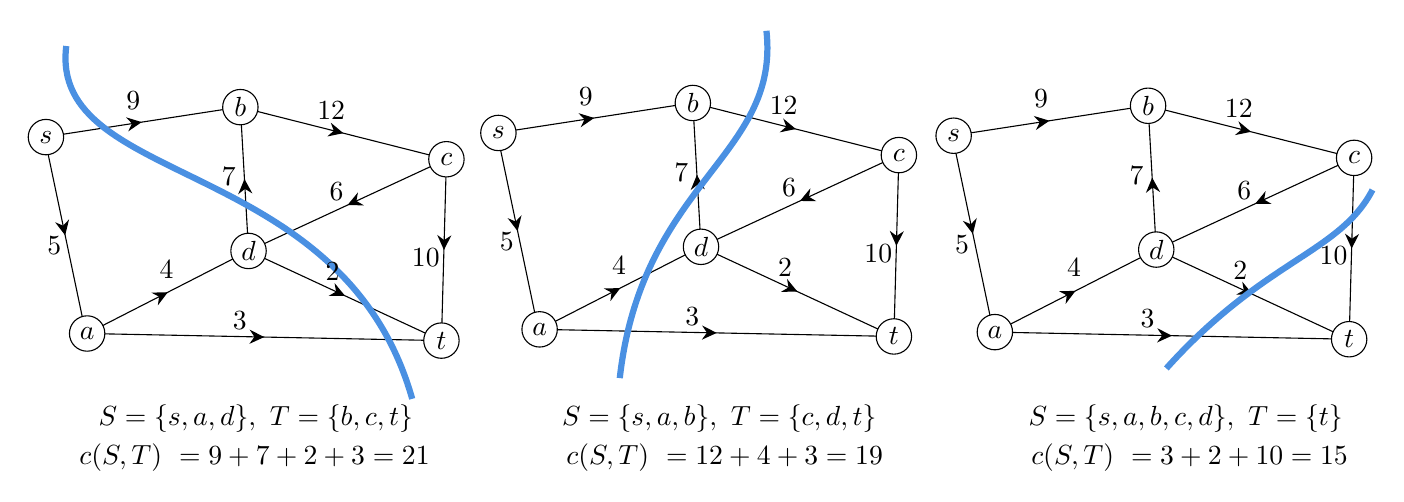
\begin{tikzpicture}[x=0.5pt,y=0.5pt,yscale=-1,xscale=1]
%uncomment if require: \path (0,338); %set diagram left start at 0, and has height of 338

%Straight Lines [id:da3853598268579197] 
\draw    (28.79,82.83) -- (169.31,61.18) ;
\draw [shift={(99.05,72)}, rotate = 531.24] [fill={rgb, 255:red, 0; green, 0; blue, 0 }  ][line width=0.08]  [draw opacity=0] (10.72,-5.15) -- (0,0) -- (10.72,5.15) -- (7.12,0) -- cycle    ;
%Straight Lines [id:da6958538828947681] 
\draw    (28.79,82.83) -- (58.58,224.77) ;
\draw [shift={(43.69,153.8)}, rotate = 258.15] [fill={rgb, 255:red, 0; green, 0; blue, 0 }  ][line width=0.08]  [draw opacity=0] (10.72,-5.15) -- (0,0) -- (10.72,5.15) -- (7.12,0) -- cycle    ;
%Straight Lines [id:da2980592918523626] 
\draw    (59.58,224.77) -- (315.62,229.9) ;
\draw [shift={(187.6,227.34)}, rotate = 181.15] [fill={rgb, 255:red, 0; green, 0; blue, 0 }  ][line width=0.08]  [draw opacity=0] (10.72,-5.15) -- (0,0) -- (10.72,5.15) -- (7.12,0) -- cycle    ;
%Straight Lines [id:da14604600957867897] 
\draw    (176.22,165.11) -- (315.62,229.9) ;
\draw [shift={(245.92,197.5)}, rotate = 204.92000000000002] [fill={rgb, 255:red, 0; green, 0; blue, 0 }  ][line width=0.08]  [draw opacity=0] (10.72,-5.15) -- (0,0) -- (10.72,5.15) -- (7.12,0) -- cycle    ;
%Straight Lines [id:da8640956582518242] 
\draw    (170.31,61.18) -- (176.22,165.11) ;
\draw [shift={(173.27,113.14)}, rotate = 86.75] [fill={rgb, 255:red, 0; green, 0; blue, 0 }  ][line width=0.08]  [draw opacity=0] (10.72,-5.15) -- (0,0) -- (10.72,5.15) -- (7.12,0) -- cycle    ;
%Straight Lines [id:da285469110869773] 
\draw    (170.31,61.18) -- (319.22,98.84) ;
\draw [shift={(244.76,80.01)}, rotate = 194.2] [fill={rgb, 255:red, 0; green, 0; blue, 0 }  ][line width=0.08]  [draw opacity=0] (10.72,-5.15) -- (0,0) -- (10.72,5.15) -- (7.12,0) -- cycle    ;
%Straight Lines [id:da8162300663234149] 
\draw    (319.22,98.84) -- (315.62,229.9) ;
\draw [shift={(317.42,164.37)}, rotate = 271.57] [fill={rgb, 255:red, 0; green, 0; blue, 0 }  ][line width=0.08]  [draw opacity=0] (10.72,-5.15) -- (0,0) -- (10.72,5.15) -- (7.12,0) -- cycle    ;
%Straight Lines [id:da5085854502811855] 
\draw    (319.22,98.84) -- (176.22,165.11) ;
\draw [shift={(247.72,131.98)}, rotate = 335.13] [fill={rgb, 255:red, 0; green, 0; blue, 0 }  ][line width=0.08]  [draw opacity=0] (10.72,-5.15) -- (0,0) -- (10.72,5.15) -- (7.12,0) -- cycle    ;
%Straight Lines [id:da4064365628912957] 
\draw    (176.22,165.11) -- (59.58,224.77) ;
\draw [shift={(117.9,194.94)}, rotate = 152.91] [fill={rgb, 255:red, 0; green, 0; blue, 0 }  ][line width=0.08]  [draw opacity=0] (10.72,-5.15) -- (0,0) -- (10.72,5.15) -- (7.12,0) -- cycle    ;
%Shape: Ellipse [id:dp651117123053256] 
\draw  [fill={rgb, 255:red, 255; green, 255; blue, 255 }  ,fill opacity=1 ] (17,82.83) .. controls (17,75.77) and (22.73,70.04) .. (29.79,70.04) .. controls (36.86,70.04) and (42.58,75.77) .. (42.58,82.83) .. controls (42.58,89.9) and (36.86,95.62) .. (29.79,95.62) .. controls (22.73,95.62) and (17,89.9) .. (17,82.83) -- cycle ;
%Shape: Ellipse [id:dp7399561756845123] 
\draw  [fill={rgb, 255:red, 255; green, 255; blue, 255 }  ,fill opacity=1 ] (157.52,61.18) .. controls (157.52,54.11) and (163.25,48.39) .. (170.31,48.39) .. controls (177.38,48.39) and (183.1,54.11) .. (183.1,61.18) .. controls (183.1,68.24) and (177.38,73.97) .. (170.31,73.97) .. controls (163.25,73.97) and (157.52,68.24) .. (157.52,61.18) -- cycle ;
%Shape: Ellipse [id:dp8268258265249401] 
\draw  [fill={rgb, 255:red, 255; green, 255; blue, 255 }  ,fill opacity=1 ] (306.43,98.84) .. controls (306.43,91.78) and (312.15,86.05) .. (319.22,86.05) .. controls (326.28,86.05) and (332.01,91.78) .. (332.01,98.84) .. controls (332.01,105.9) and (326.28,111.63) .. (319.22,111.63) .. controls (312.15,111.63) and (306.43,105.9) .. (306.43,98.84) -- cycle ;
%Shape: Ellipse [id:dp5421818862330341] 
\draw  [fill={rgb, 255:red, 255; green, 255; blue, 255 }  ,fill opacity=1 ] (163.43,165.11) .. controls (163.43,158.05) and (169.15,152.32) .. (176.22,152.32) .. controls (183.28,152.32) and (189.01,158.05) .. (189.01,165.11) .. controls (189.01,172.18) and (183.28,177.9) .. (176.22,177.9) .. controls (169.15,177.9) and (163.43,172.18) .. (163.43,165.11) -- cycle ;
%Shape: Ellipse [id:dp45600813719389455] 
\draw  [fill={rgb, 255:red, 255; green, 255; blue, 255 }  ,fill opacity=1 ] (46.79,224.77) .. controls (46.79,217.71) and (52.52,211.98) .. (59.58,211.98) .. controls (66.64,211.98) and (72.37,217.71) .. (72.37,224.77) .. controls (72.37,231.84) and (66.64,237.56) .. (59.58,237.56) .. controls (52.52,237.56) and (46.79,231.84) .. (46.79,224.77) -- cycle ;
%Shape: Ellipse [id:dp031187496945339066] 
\draw  [fill={rgb, 255:red, 255; green, 255; blue, 255 }  ,fill opacity=1 ] (302.83,229.9) .. controls (302.83,222.83) and (308.56,217.11) .. (315.62,217.11) .. controls (322.69,217.11) and (328.41,222.83) .. (328.41,229.9) .. controls (328.41,236.96) and (322.69,242.69) .. (315.62,242.69) .. controls (308.56,242.69) and (302.83,236.96) .. (302.83,229.9) -- cycle ;
%Straight Lines [id:da7435046067409884] 
\draw    (355.79,79.83) -- (496.31,58.18) ;
\draw [shift={(426.05,69)}, rotate = 531.24] [fill={rgb, 255:red, 0; green, 0; blue, 0 }  ][line width=0.08]  [draw opacity=0] (10.72,-5.15) -- (0,0) -- (10.72,5.15) -- (7.12,0) -- cycle    ;
%Straight Lines [id:da8387107518837462] 
\draw    (355.79,79.83) -- (385.58,221.77) ;
\draw [shift={(370.69,150.8)}, rotate = 258.15] [fill={rgb, 255:red, 0; green, 0; blue, 0 }  ][line width=0.08]  [draw opacity=0] (10.72,-5.15) -- (0,0) -- (10.72,5.15) -- (7.12,0) -- cycle    ;
%Straight Lines [id:da3219489964495771] 
\draw    (386.58,221.77) -- (642.62,226.9) ;
\draw [shift={(514.6,224.34)}, rotate = 181.15] [fill={rgb, 255:red, 0; green, 0; blue, 0 }  ][line width=0.08]  [draw opacity=0] (10.72,-5.15) -- (0,0) -- (10.72,5.15) -- (7.12,0) -- cycle    ;
%Straight Lines [id:da7100151765093478] 
\draw    (503.22,162.11) -- (642.62,226.9) ;
\draw [shift={(572.92,194.5)}, rotate = 204.92000000000002] [fill={rgb, 255:red, 0; green, 0; blue, 0 }  ][line width=0.08]  [draw opacity=0] (10.72,-5.15) -- (0,0) -- (10.72,5.15) -- (7.12,0) -- cycle    ;
%Straight Lines [id:da4338060480266903] 
\draw    (497.31,58.18) -- (503.22,162.11) ;
\draw [shift={(500.27,110.14)}, rotate = 86.75] [fill={rgb, 255:red, 0; green, 0; blue, 0 }  ][line width=0.08]  [draw opacity=0] (10.72,-5.15) -- (0,0) -- (10.72,5.15) -- (7.12,0) -- cycle    ;
%Straight Lines [id:da7182225488033221] 
\draw    (497.31,58.18) -- (646.22,95.84) ;
\draw [shift={(571.76,77.01)}, rotate = 194.2] [fill={rgb, 255:red, 0; green, 0; blue, 0 }  ][line width=0.08]  [draw opacity=0] (10.72,-5.15) -- (0,0) -- (10.72,5.15) -- (7.12,0) -- cycle    ;
%Straight Lines [id:da5940568426447731] 
\draw    (646.22,95.84) -- (642.62,226.9) ;
\draw [shift={(644.42,161.37)}, rotate = 271.57] [fill={rgb, 255:red, 0; green, 0; blue, 0 }  ][line width=0.08]  [draw opacity=0] (10.72,-5.15) -- (0,0) -- (10.72,5.15) -- (7.12,0) -- cycle    ;
%Straight Lines [id:da6584403815712339] 
\draw    (646.22,95.84) -- (503.22,162.11) ;
\draw [shift={(574.72,128.98)}, rotate = 335.13] [fill={rgb, 255:red, 0; green, 0; blue, 0 }  ][line width=0.08]  [draw opacity=0] (10.72,-5.15) -- (0,0) -- (10.72,5.15) -- (7.12,0) -- cycle    ;
%Straight Lines [id:da04611791534207066] 
\draw    (503.22,162.11) -- (386.58,221.77) ;
\draw [shift={(444.9,191.94)}, rotate = 152.91] [fill={rgb, 255:red, 0; green, 0; blue, 0 }  ][line width=0.08]  [draw opacity=0] (10.72,-5.15) -- (0,0) -- (10.72,5.15) -- (7.12,0) -- cycle    ;
%Shape: Ellipse [id:dp8684805017046724] 
\draw  [fill={rgb, 255:red, 255; green, 255; blue, 255 }  ,fill opacity=1 ] (344,79.83) .. controls (344,72.77) and (349.73,67.04) .. (356.79,67.04) .. controls (363.86,67.04) and (369.58,72.77) .. (369.58,79.83) .. controls (369.58,86.9) and (363.86,92.62) .. (356.79,92.62) .. controls (349.73,92.62) and (344,86.9) .. (344,79.83) -- cycle ;
%Shape: Ellipse [id:dp26598537007129874] 
\draw  [fill={rgb, 255:red, 255; green, 255; blue, 255 }  ,fill opacity=1 ] (484.52,58.18) .. controls (484.52,51.11) and (490.25,45.39) .. (497.31,45.39) .. controls (504.38,45.39) and (510.1,51.11) .. (510.1,58.18) .. controls (510.1,65.24) and (504.38,70.97) .. (497.31,70.97) .. controls (490.25,70.97) and (484.52,65.24) .. (484.52,58.18) -- cycle ;
%Shape: Ellipse [id:dp8446989445980774] 
\draw  [fill={rgb, 255:red, 255; green, 255; blue, 255 }  ,fill opacity=1 ] (633.43,95.84) .. controls (633.43,88.78) and (639.15,83.05) .. (646.22,83.05) .. controls (653.28,83.05) and (659.01,88.78) .. (659.01,95.84) .. controls (659.01,102.9) and (653.28,108.63) .. (646.22,108.63) .. controls (639.15,108.63) and (633.43,102.9) .. (633.43,95.84) -- cycle ;
%Shape: Ellipse [id:dp5784359228600563] 
\draw  [fill={rgb, 255:red, 255; green, 255; blue, 255 }  ,fill opacity=1 ] (490.43,162.11) .. controls (490.43,155.05) and (496.15,149.32) .. (503.22,149.32) .. controls (510.28,149.32) and (516.01,155.05) .. (516.01,162.11) .. controls (516.01,169.18) and (510.28,174.9) .. (503.22,174.9) .. controls (496.15,174.9) and (490.43,169.18) .. (490.43,162.11) -- cycle ;
%Shape: Ellipse [id:dp971944601404772] 
\draw  [fill={rgb, 255:red, 255; green, 255; blue, 255 }  ,fill opacity=1 ] (373.79,221.77) .. controls (373.79,214.71) and (379.52,208.98) .. (386.58,208.98) .. controls (393.64,208.98) and (399.37,214.71) .. (399.37,221.77) .. controls (399.37,228.84) and (393.64,234.56) .. (386.58,234.56) .. controls (379.52,234.56) and (373.79,228.84) .. (373.79,221.77) -- cycle ;
%Shape: Ellipse [id:dp1835030596812679] 
\draw  [fill={rgb, 255:red, 255; green, 255; blue, 255 }  ,fill opacity=1 ] (629.83,226.9) .. controls (629.83,219.83) and (635.56,214.11) .. (642.62,214.11) .. controls (649.69,214.11) and (655.41,219.83) .. (655.41,226.9) .. controls (655.41,233.96) and (649.69,239.69) .. (642.62,239.69) .. controls (635.56,239.69) and (629.83,233.96) .. (629.83,226.9) -- cycle ;
%Curve Lines [id:da2649473788057739] 
\draw [color={rgb, 255:red, 74; green, 144; blue, 226 }  ,draw opacity=1 ][line width=2.25]    (44.5,17) .. controls (31.5,120) and (244.5,95) .. (294.5,272) ;
%Curve Lines [id:da16888389279841676] 
\draw [color={rgb, 255:red, 74; green, 144; blue, 226 }  ,draw opacity=1 ][line width=2.25]    (550.5,6) .. controls (560.5,97) and (460.5,115) .. (444.5,257) ;
%Straight Lines [id:da23959710765930176] 
\draw    (684.79,81.83) -- (825.31,60.18) ;
\draw [shift={(755.05,71)}, rotate = 531.24] [fill={rgb, 255:red, 0; green, 0; blue, 0 }  ][line width=0.08]  [draw opacity=0] (10.72,-5.15) -- (0,0) -- (10.72,5.15) -- (7.12,0) -- cycle    ;
%Straight Lines [id:da6431206981927323] 
\draw    (684.79,81.83) -- (714.58,223.77) ;
\draw [shift={(699.69,152.8)}, rotate = 258.15] [fill={rgb, 255:red, 0; green, 0; blue, 0 }  ][line width=0.08]  [draw opacity=0] (10.72,-5.15) -- (0,0) -- (10.72,5.15) -- (7.12,0) -- cycle    ;
%Straight Lines [id:da5596554414836099] 
\draw    (715.58,223.77) -- (971.62,228.9) ;
\draw [shift={(843.6,226.34)}, rotate = 181.15] [fill={rgb, 255:red, 0; green, 0; blue, 0 }  ][line width=0.08]  [draw opacity=0] (10.72,-5.15) -- (0,0) -- (10.72,5.15) -- (7.12,0) -- cycle    ;
%Straight Lines [id:da8160720971935526] 
\draw    (832.22,164.11) -- (971.62,228.9) ;
\draw [shift={(901.92,196.5)}, rotate = 204.92000000000002] [fill={rgb, 255:red, 0; green, 0; blue, 0 }  ][line width=0.08]  [draw opacity=0] (10.72,-5.15) -- (0,0) -- (10.72,5.15) -- (7.12,0) -- cycle    ;
%Straight Lines [id:da3877819200248832] 
\draw    (826.31,60.18) -- (832.22,164.11) ;
\draw [shift={(829.27,112.14)}, rotate = 86.75] [fill={rgb, 255:red, 0; green, 0; blue, 0 }  ][line width=0.08]  [draw opacity=0] (10.72,-5.15) -- (0,0) -- (10.72,5.15) -- (7.12,0) -- cycle    ;
%Straight Lines [id:da057104792707504015] 
\draw    (826.31,60.18) -- (975.22,97.84) ;
\draw [shift={(900.76,79.01)}, rotate = 194.2] [fill={rgb, 255:red, 0; green, 0; blue, 0 }  ][line width=0.08]  [draw opacity=0] (10.72,-5.15) -- (0,0) -- (10.72,5.15) -- (7.12,0) -- cycle    ;
%Straight Lines [id:da14831136034761006] 
\draw    (975.22,97.84) -- (971.62,228.9) ;
\draw [shift={(973.42,163.37)}, rotate = 271.57] [fill={rgb, 255:red, 0; green, 0; blue, 0 }  ][line width=0.08]  [draw opacity=0] (10.72,-5.15) -- (0,0) -- (10.72,5.15) -- (7.12,0) -- cycle    ;
%Straight Lines [id:da2506057291921263] 
\draw    (975.22,97.84) -- (832.22,164.11) ;
\draw [shift={(903.72,130.98)}, rotate = 335.13] [fill={rgb, 255:red, 0; green, 0; blue, 0 }  ][line width=0.08]  [draw opacity=0] (10.72,-5.15) -- (0,0) -- (10.72,5.15) -- (7.12,0) -- cycle    ;
%Straight Lines [id:da7375159787579277] 
\draw    (832.22,164.11) -- (715.58,223.77) ;
\draw [shift={(773.9,193.94)}, rotate = 152.91] [fill={rgb, 255:red, 0; green, 0; blue, 0 }  ][line width=0.08]  [draw opacity=0] (10.72,-5.15) -- (0,0) -- (10.72,5.15) -- (7.12,0) -- cycle    ;
%Shape: Ellipse [id:dp7941672492891375] 
\draw  [fill={rgb, 255:red, 255; green, 255; blue, 255 }  ,fill opacity=1 ] (673,81.83) .. controls (673,74.77) and (678.73,69.04) .. (685.79,69.04) .. controls (692.86,69.04) and (698.58,74.77) .. (698.58,81.83) .. controls (698.58,88.9) and (692.86,94.62) .. (685.79,94.62) .. controls (678.73,94.62) and (673,88.9) .. (673,81.83) -- cycle ;
%Shape: Ellipse [id:dp3757660056746118] 
\draw  [fill={rgb, 255:red, 255; green, 255; blue, 255 }  ,fill opacity=1 ] (813.52,60.18) .. controls (813.52,53.11) and (819.25,47.39) .. (826.31,47.39) .. controls (833.38,47.39) and (839.1,53.11) .. (839.1,60.18) .. controls (839.1,67.24) and (833.38,72.97) .. (826.31,72.97) .. controls (819.25,72.97) and (813.52,67.24) .. (813.52,60.18) -- cycle ;
%Shape: Ellipse [id:dp9316219699822907] 
\draw  [fill={rgb, 255:red, 255; green, 255; blue, 255 }  ,fill opacity=1 ] (962.43,97.84) .. controls (962.43,90.78) and (968.15,85.05) .. (975.22,85.05) .. controls (982.28,85.05) and (988.01,90.78) .. (988.01,97.84) .. controls (988.01,104.9) and (982.28,110.63) .. (975.22,110.63) .. controls (968.15,110.63) and (962.43,104.9) .. (962.43,97.84) -- cycle ;
%Shape: Ellipse [id:dp2713572714021609] 
\draw  [fill={rgb, 255:red, 255; green, 255; blue, 255 }  ,fill opacity=1 ] (819.43,164.11) .. controls (819.43,157.05) and (825.15,151.32) .. (832.22,151.32) .. controls (839.28,151.32) and (845.01,157.05) .. (845.01,164.11) .. controls (845.01,171.18) and (839.28,176.9) .. (832.22,176.9) .. controls (825.15,176.9) and (819.43,171.18) .. (819.43,164.11) -- cycle ;
%Shape: Ellipse [id:dp8303944409855877] 
\draw  [fill={rgb, 255:red, 255; green, 255; blue, 255 }  ,fill opacity=1 ] (702.79,223.77) .. controls (702.79,216.71) and (708.52,210.98) .. (715.58,210.98) .. controls (722.64,210.98) and (728.37,216.71) .. (728.37,223.77) .. controls (728.37,230.84) and (722.64,236.56) .. (715.58,236.56) .. controls (708.52,236.56) and (702.79,230.84) .. (702.79,223.77) -- cycle ;
%Shape: Ellipse [id:dp3672414292204079] 
\draw  [fill={rgb, 255:red, 255; green, 255; blue, 255 }  ,fill opacity=1 ] (958.83,228.9) .. controls (958.83,221.83) and (964.56,216.11) .. (971.62,216.11) .. controls (978.69,216.11) and (984.41,221.83) .. (984.41,228.9) .. controls (984.41,235.96) and (978.69,241.69) .. (971.62,241.69) .. controls (964.56,241.69) and (958.83,235.96) .. (958.83,228.9) -- cycle ;
%Curve Lines [id:da42045420214553086] 
\draw [color={rgb, 255:red, 74; green, 144; blue, 226 }  ,draw opacity=1 ][line width=2.25]    (988.5,121) .. controls (964.5,167) and (910.5,171) .. (839.5,250) ;

% Text Node
\draw (29.79,82.83) node   [align=left] {$\displaystyle s$};
% Text Node
\draw (170.31,61.18) node   [align=left] {$\displaystyle b$};
% Text Node
\draw (319.22,98.84) node   [align=left] {$\displaystyle c$};
% Text Node
\draw (176.22,165.11) node   [align=left] {$\displaystyle d$};
% Text Node
\draw (59.58,224.77) node   [align=left] {$\displaystyle a$};
% Text Node
\draw (315.62,229.9) node   [align=left] {$\displaystyle t$};
% Text Node
\draw (29,153) node [anchor=north west][inner sep=0.75pt]   [align=left] {$\displaystyle 5$};
% Text Node
\draw (110,170) node [anchor=north west][inner sep=0.75pt]   [align=left] {$\displaystyle 4$};
% Text Node
\draw (86,48) node [anchor=north west][inner sep=0.75pt]   [align=left] {$\displaystyle 9$};
% Text Node
\draw (233,114) node [anchor=north west][inner sep=0.75pt]   [align=left] {$\displaystyle 6$};
% Text Node
\draw (155,103) node [anchor=north west][inner sep=0.75pt]   [align=left] {$\displaystyle 7$};
% Text Node
\draw (230,172) node [anchor=north west][inner sep=0.75pt]   [align=left] {$\displaystyle 2$};
% Text Node
\draw (292.42,161.37) node [anchor=north west][inner sep=0.75pt]   [align=left] {$\displaystyle 10$};
% Text Node
\draw (224,55) node [anchor=north west][inner sep=0.75pt]   [align=left] {$\displaystyle 12$};
% Text Node
\draw (163,207) node [anchor=north west][inner sep=0.75pt]   [align=left] {$\displaystyle 3$};
% Text Node
\draw (356.79,79.83) node   [align=left] {$\displaystyle s$};
% Text Node
\draw (497.31,58.18) node   [align=left] {$\displaystyle b$};
% Text Node
\draw (646.22,95.84) node   [align=left] {$\displaystyle c$};
% Text Node
\draw (503.22,162.11) node   [align=left] {$\displaystyle d$};
% Text Node
\draw (386.58,221.77) node   [align=left] {$\displaystyle a$};
% Text Node
\draw (642.62,226.9) node   [align=left] {$\displaystyle t$};
% Text Node
\draw (356,150) node [anchor=north west][inner sep=0.75pt]   [align=left] {$\displaystyle 5$};
% Text Node
\draw (437,167) node [anchor=north west][inner sep=0.75pt]   [align=left] {$\displaystyle 4$};
% Text Node
\draw (413,45) node [anchor=north west][inner sep=0.75pt]   [align=left] {$\displaystyle 9$};
% Text Node
\draw (560,111) node [anchor=north west][inner sep=0.75pt]   [align=left] {$\displaystyle 6$};
% Text Node
\draw (482,100) node [anchor=north west][inner sep=0.75pt]   [align=left] {$\displaystyle 7$};
% Text Node
\draw (557,169) node [anchor=north west][inner sep=0.75pt]   [align=left] {$\displaystyle 2$};
% Text Node
\draw (619.42,158.37) node [anchor=north west][inner sep=0.75pt]   [align=left] {$\displaystyle 10$};
% Text Node
\draw (551,52) node [anchor=north west][inner sep=0.75pt]   [align=left] {$\displaystyle 12$};
% Text Node
\draw (490,204) node [anchor=north west][inner sep=0.75pt]   [align=left] {$\displaystyle 3$};
% Text Node
\draw (52,302.5) node [anchor=north west][inner sep=0.75pt]   [align=left] {$\displaystyle c( S,T) \ =9+7+2+3=21$};
% Text Node
\draw (404,302.5) node [anchor=north west][inner sep=0.75pt]   [align=left] {$\displaystyle c( S,T) \ =12+4+3=19$};
% Text Node
\draw (685.79,81.83) node   [align=left] {$\displaystyle s$};
% Text Node
\draw (826.31,60.18) node   [align=left] {$\displaystyle b$};
% Text Node
\draw (975.22,97.84) node   [align=left] {$\displaystyle c$};
% Text Node
\draw (832.22,164.11) node   [align=left] {$\displaystyle d$};
% Text Node
\draw (715.58,223.77) node   [align=left] {$\displaystyle a$};
% Text Node
\draw (971.62,228.9) node   [align=left] {$\displaystyle t$};
% Text Node
\draw (685,152) node [anchor=north west][inner sep=0.75pt]   [align=left] {$\displaystyle 5$};
% Text Node
\draw (766,169) node [anchor=north west][inner sep=0.75pt]   [align=left] {$\displaystyle 4$};
% Text Node
\draw (742,47) node [anchor=north west][inner sep=0.75pt]   [align=left] {$\displaystyle 9$};
% Text Node
\draw (889,113) node [anchor=north west][inner sep=0.75pt]   [align=left] {$\displaystyle 6$};
% Text Node
\draw (811,102) node [anchor=north west][inner sep=0.75pt]   [align=left] {$\displaystyle 7$};
% Text Node
\draw (886,171) node [anchor=north west][inner sep=0.75pt]   [align=left] {$\displaystyle 2$};
% Text Node
\draw (948.42,160.37) node [anchor=north west][inner sep=0.75pt]   [align=left] {$\displaystyle 10$};
% Text Node
\draw (880,54) node [anchor=north west][inner sep=0.75pt]   [align=left] {$\displaystyle 12$};
% Text Node
\draw (819,206) node [anchor=north west][inner sep=0.75pt]   [align=left] {$\displaystyle 3$};
% Text Node
\draw (740,302.5) node [anchor=north west][inner sep=0.75pt]   [align=left] {$\displaystyle c( S,T) \ =3+2+10=15$};
% Text Node
\draw (66,274.5) node [anchor=north west][inner sep=0.75pt]   [align=left] {$\displaystyle S=\{s,a,d\} ,\ T=\{b,c,t\}$};
% Text Node
\draw (401,274.5) node [anchor=north west][inner sep=0.75pt]   [align=left] {$\displaystyle S=\{s,a,b\} ,\ T=\{c,d,t\}$};
% Text Node
\draw (738,274.5) node [anchor=north west][inner sep=0.75pt]   [align=left] {$\displaystyle S=\{s,a,b,c,d\} ,\ T=\{t\}$};


\end{tikzpicture}

}
\caption{Four different $s$-$t$ cuts and their capacities of the same network.}
\label{fig:flow-cut}
\end{figure}

We now introduce the so-called \emph{minimum-cut problem}: given network $G = (V, E)$ with source $s$, sink $t$ and capacity $c(e)$ for any $e\in E$,
   we seek an $s$-$t$ cut $(S, T)$ such that its capacity $c(S, T)$ is minimized.

Note that, the definition of $s$-$t$ cut, capacity of an $s$-$t$ cut, and above minimum-cut problem,
are completely independent of flow. Note too that, the input of the maximum-flow problem and the minimum-cut
problem is the same: a network~(consisting of a directed graph, source and sink, and edge capacities).

Although the maximum-flow problem and the minimum-cut problem are defined independently, they
can be solved by the same algorithm~(for example, the Ford-Fulkson algorithm)
and are connected by an elegant theorem~(i.e., the max-flow min-cut theorem).
Below, we first show half of this theorem.
Later on we will introduce the Ford-Fulkson algorithm
and use it to prove the other other half of the theorem.

%\subsection*{Maximum-Flow v.s.\ Minimum-Cut, One-Side Connection}

We now show that, the capacity of \emph{any} $s$-$t$ cut of a network
gives an \emph{upper bound} of the value of \emph{any} $s$-$t$ flow of the same network, 
formally stated below.
\begin{claim} \label{claim1}
Let $(G=(V, E), s, t, c(\cdot))$ be a network.
Let $f$ be an arbitrary $s$-$t$ flow and let $(S, T)$ be an arbitrary $s$-$t$ cut, of this network.
We have $|f| \le c(S, T)$.
\end{claim}

Above claim is intuitive to understand: an $s$-$t$ flow $f$ transfer $|f|$ units of flow from source $s$ to sink $t$;
since an $s$-$t$ cut $(S, T)$ separates $s$ and $t$, so the flow, all generated from $s$, must cross the cut in order to reach $t$,
and such ``crossing'' must use the cut-edges.
Hence, the total amount of the flow that can be transferred, i.e., the value of $f$, is limitted by
the total capacities of the cut-edges, i.e., the capacity of the $s$-$t$ cut.
See Figure~\ref{fig:claim}.

\begin{figure}[h]
\centering{

\tikzset{every picture/.style={line width=0.75pt}} %set default line width to 0.75pt        

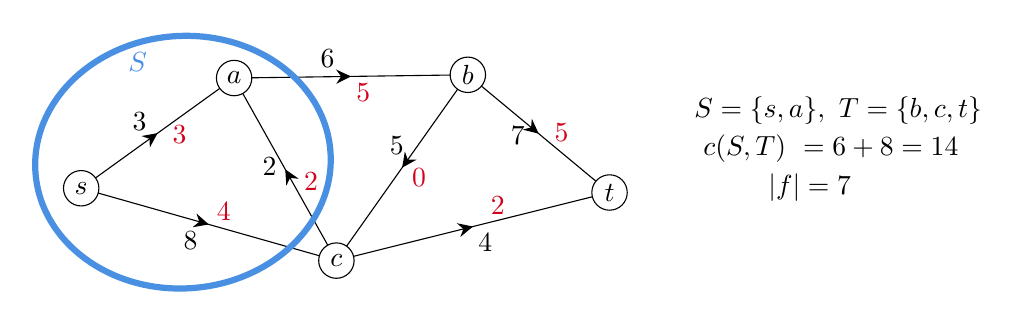
\begin{tikzpicture}[x=0.5pt,y=0.5pt,yscale=-1,xscale=1]
%uncomment if require: \path (0,210); %set diagram left start at 0, and has height of 210

%Straight Lines [id:da31781895407498073] 
\draw    (227.22,173.11) -- (322.22,38.84) ;
\draw [shift={(274.72,105.98)}, rotate = 305.28] [fill={rgb, 255:red, 0; green, 0; blue, 0 }  ][line width=0.08]  [draw opacity=0] (10.72,-5.15) -- (0,0) -- (10.72,5.15) -- (7.12,0) -- cycle    ;
%Straight Lines [id:da3853598268579197] 
\draw    (153.31,41.18) -- (227.22,173.11) ;
\draw [shift={(190.27,107.14)}, rotate = 60.74] [fill={rgb, 255:red, 0; green, 0; blue, 0 }  ][line width=0.08]  [draw opacity=0] (10.72,-5.15) -- (0,0) -- (10.72,5.15) -- (7.12,0) -- cycle    ;
%Straight Lines [id:da14604600957867897] 
\draw    (42.79,120.83) -- (227.22,173.11) ;
\draw [shift={(135.01,146.97)}, rotate = 195.83] [fill={rgb, 255:red, 0; green, 0; blue, 0 }  ][line width=0.08]  [draw opacity=0] (10.72,-5.15) -- (0,0) -- (10.72,5.15) -- (7.12,0) -- cycle    ;
%Straight Lines [id:da8640956582518242] 
\draw    (424.62,123.9) -- (227.22,173.11) ;
\draw [shift={(325.92,148.5)}, rotate = 166] [fill={rgb, 255:red, 0; green, 0; blue, 0 }  ][line width=0.08]  [draw opacity=0] (10.72,-5.15) -- (0,0) -- (10.72,5.15) -- (7.12,0) -- cycle    ;
%Straight Lines [id:da285469110869773] 
\draw    (42.79,120.83) -- (153.31,41.18) ;
\draw [shift={(98.05,81)}, rotate = 504.22] [fill={rgb, 255:red, 0; green, 0; blue, 0 }  ][line width=0.08]  [draw opacity=0] (10.72,-5.15) -- (0,0) -- (10.72,5.15) -- (7.12,0) -- cycle    ;
%Straight Lines [id:da8162300663234149] 
\draw    (322.22,38.84) -- (424.62,123.9) ;
\draw [shift={(373.42,81.37)}, rotate = 219.71] [fill={rgb, 255:red, 0; green, 0; blue, 0 }  ][line width=0.08]  [draw opacity=0] (10.72,-5.15) -- (0,0) -- (10.72,5.15) -- (7.12,0) -- cycle    ;
%Straight Lines [id:da5085854502811855] 
\draw    (153.31,41.18) -- (322.22,38.84) ;
\draw [shift={(237.76,40.01)}, rotate = 539.21] [fill={rgb, 255:red, 0; green, 0; blue, 0 }  ][line width=0.08]  [draw opacity=0] (10.72,-5.15) -- (0,0) -- (10.72,5.15) -- (7.12,0) -- cycle    ;
%Shape: Ellipse [id:dp651117123053256] 
\draw  [fill={rgb, 255:red, 255; green, 255; blue, 255 }  ,fill opacity=1 ] (30,120.83) .. controls (30,113.77) and (35.73,108.04) .. (42.79,108.04) .. controls (49.86,108.04) and (55.58,113.77) .. (55.58,120.83) .. controls (55.58,127.9) and (49.86,133.62) .. (42.79,133.62) .. controls (35.73,133.62) and (30,127.9) .. (30,120.83) -- cycle ;
%Shape: Ellipse [id:dp7399561756845123] 
\draw  [fill={rgb, 255:red, 255; green, 255; blue, 255 }  ,fill opacity=1 ] (140.52,41.18) .. controls (140.52,34.11) and (146.25,28.39) .. (153.31,28.39) .. controls (160.38,28.39) and (166.1,34.11) .. (166.1,41.18) .. controls (166.1,48.24) and (160.38,53.97) .. (153.31,53.97) .. controls (146.25,53.97) and (140.52,48.24) .. (140.52,41.18) -- cycle ;
%Shape: Ellipse [id:dp8268258265249401] 
\draw  [fill={rgb, 255:red, 255; green, 255; blue, 255 }  ,fill opacity=1 ] (309.43,38.84) .. controls (309.43,31.78) and (315.15,26.05) .. (322.22,26.05) .. controls (329.28,26.05) and (335.01,31.78) .. (335.01,38.84) .. controls (335.01,45.9) and (329.28,51.63) .. (322.22,51.63) .. controls (315.15,51.63) and (309.43,45.9) .. (309.43,38.84) -- cycle ;
%Shape: Ellipse [id:dp5421818862330341] 
\draw  [fill={rgb, 255:red, 255; green, 255; blue, 255 }  ,fill opacity=1 ] (214.43,173.11) .. controls (214.43,166.05) and (220.15,160.32) .. (227.22,160.32) .. controls (234.28,160.32) and (240.01,166.05) .. (240.01,173.11) .. controls (240.01,180.18) and (234.28,185.9) .. (227.22,185.9) .. controls (220.15,185.9) and (214.43,180.18) .. (214.43,173.11) -- cycle ;
%Shape: Ellipse [id:dp031187496945339066] 
\draw  [fill={rgb, 255:red, 255; green, 255; blue, 255 }  ,fill opacity=1 ] (411.83,123.9) .. controls (411.83,116.83) and (417.56,111.11) .. (424.62,111.11) .. controls (431.69,111.11) and (437.41,116.83) .. (437.41,123.9) .. controls (437.41,130.96) and (431.69,136.69) .. (424.62,136.69) .. controls (417.56,136.69) and (411.83,130.96) .. (411.83,123.9) -- cycle ;
%Shape: Ellipse [id:dp3896768851761181] 
\draw  [color={rgb, 255:red, 74; green, 144; blue, 226 }  ,draw opacity=1 ][line width=2.25]  (110.27,10.95) .. controls (169.16,7.03) and (219.61,44.6) .. (222.96,94.88) .. controls (226.31,145.15) and (181.28,189.09) .. (122.39,193.01) .. controls (63.51,196.93) and (13.05,159.35) .. (9.71,109.08) .. controls (6.36,58.8) and (51.38,14.87) .. (110.27,10.95) -- cycle ;

% Text Node
\draw (42.79,120.83) node   [align=left] {$\displaystyle s$};
% Text Node
\draw (153.31,41.18) node   [align=left] {$\displaystyle a$};
% Text Node
\draw (322.22,38.84) node   [align=left] {$\displaystyle b$};
% Text Node
\draw (227.22,173.11) node   [align=left] {$\displaystyle c$};
% Text Node
\draw (424.62,123.9) node   [align=left] {$\displaystyle t$};
% Text Node
\draw (115,150) node [anchor=north west][inner sep=0.75pt]   [align=left] {$\displaystyle 8$};
% Text Node
\draw (264,82) node [anchor=north west][inner sep=0.75pt]   [align=left] {$\displaystyle 5$};
% Text Node
\draw (172,97) node [anchor=north west][inner sep=0.75pt]   [align=left] {$\displaystyle 2$};
% Text Node
\draw (78,64) node [anchor=north west][inner sep=0.75pt]   [align=left] {$\displaystyle 3$};
% Text Node
\draw (327.92,151.5) node [anchor=north west][inner sep=0.75pt]   [align=left] {$\displaystyle 4$};
% Text Node
\draw (351.42,74.37) node [anchor=north west][inner sep=0.75pt]   [align=left] {$\displaystyle 7$};
% Text Node
\draw (214,19) node [anchor=north west][inner sep=0.75pt]   [align=left] {$\displaystyle 6$};
% Text Node
\draw (490.5,80.5) node [anchor=north west][inner sep=0.75pt]   [align=left] {$\displaystyle c( S,T) \ =6+8=14$};
% Text Node
\draw (484,52.5) node [anchor=north west][inner sep=0.75pt]   [align=left] {$\displaystyle S=\{s,a\} ,\ T=\{b,c,t\}$};
% Text Node
\draw (139,129) node [anchor=north west][inner sep=0.75pt]   [align=left] {$\displaystyle \textcolor[rgb]{0.82,0.01,0.11}{4}$};
% Text Node
\draw (202,108) node [anchor=north west][inner sep=0.75pt]   [align=left] {$\displaystyle \textcolor[rgb]{0.82,0.01,0.11}{2}$};
% Text Node
\draw (337,125) node [anchor=north west][inner sep=0.75pt]   [align=left] {$\displaystyle \textcolor[rgb]{0.82,0.01,0.11}{2}$};
% Text Node
\draw (107,74) node [anchor=north west][inner sep=0.75pt]   [align=left] {$\displaystyle \textcolor[rgb]{0.82,0.01,0.11}{3}$};
% Text Node
\draw (239.76,43.01) node [anchor=north west][inner sep=0.75pt]   [align=left] {$\displaystyle \textcolor[rgb]{0.82,0.01,0.11}{5}$};
% Text Node
\draw (280,105) node [anchor=north west][inner sep=0.75pt]   [align=left] {$\displaystyle \textcolor[rgb]{0.82,0.01,0.11}{0}$};
% Text Node
\draw (383,72) node [anchor=north west][inner sep=0.75pt]   [align=left] {$\displaystyle \textcolor[rgb]{0.82,0.01,0.11}{5}$};
% Text Node
\draw (537.5,108.5) node [anchor=north west][inner sep=0.75pt]   [align=left] {$\displaystyle | f|=7$};
% Text Node
\draw (75,21) node [anchor=north west][inner sep=0.75pt]   [align=left] {$\displaystyle \textcolor[rgb]{0.29,0.56,0.89}{S}$};


\end{tikzpicture}

}
\caption{An example showing Claim~\ref{claim1} and Fact~\ref{fact1}.}
\label{fig:claim}
\end{figure}


In order to formally prove above claim, we first show that, the value of an $s$-$t$ flow $f$
can also be calculated by examining the flow carried by the ``spanning edges'' of any $s$-$t$ cut.
Formally,
\begin{fact} \label{fact1}
Let $f$ be an arbitrary $s$-$t$ flow and let $(S, T)$ be an arbitrary $s$-$t$ cut, of network $(G=(V, E), s, t, c(\cdot))$.
We have $|f| = \sum_{e\in E(S, T)} f(e) - \sum_{e\in E(T, S)} f(e)$.
\end{fact}

Above fact is also intuitive to understand: $S$ is a subset that includes $s$ but excludes $t$.
See Figure~\ref{fig:claim}.
When thinking $S$ as a whole, 
the total amount of flow generated by $S$ is equal to $|f|$, as only $s$ generates flow.
On the other hand, this amount of flow emitted from $S$ 
can also be calcuated by summing up the flow leaves $S$, i.e., $\sum_{e\in E(S, T)} f(e)$,
and subtracting the amount of the flow that enters back to $S$, i.e., $\sum_{e\in E(T, S)} f(e)$.

We now formally prove Fact~\ref{fact1}. 
Similar to the proof of Fact~1 of Lecture~36, this proof also simply applies the conservation property.

\emph{Proof of Fact~\ref{fact1}.} According to conservation property, for any $v\in S\setminus \{s\}$,
we have $\sum_{e\in I(v)} f(e) = \sum_{e\in O(v)} f(e)$. 
We sum up both sides over all $v\in S\setminus\{s\}$: 
we have $\sum_{v\in S\setminus\{s\}} \sum_{e\in I(v)} f(e) = \sum_{v\in S\setminus\{s\}} \sum_{e\in O(v)} f(e)$. 
Note that $I(s) = \emptyset$ as $s$ is a source, so the left side of above equation can be rewritten as $\sum_{v\in S} \sum_{e\in I(v)} f(e)$.
Note that $|f| = \sum_{e\in O(s)} f(e)$ by definition, so the right side can be rewritten as $\sum_{v\in S} \sum_{e\in O(v)} f(e) - |f|$.
Combined, we have $|f| = \sum_{v\in S} \sum_{e\in O(v)} f(e) - \sum_{v\in S} \sum_{e\in I(v)} f(e)$. 
Now consider the 4 types of edges partitioned by $(S, T)$ and consider if they are taken into account by the two items
i.e., $\sum_{v\in S} \sum_{e\in O(v)} f(e)$ and $\sum_{v\in S} \sum_{e\in I(v)} f(e)$. 
\vspace*{-\topsep}
\begin{enumerate}
\item All edges in $E(S, T)$ appear in the first item, but not the second one.
\item All edges in $E(T, S)$ appear in the second item, but not the first one.
\item All edges in $E(S, S)$ appear in both items~(so they cancel out).
\item None of the edges in $E(T, T)$ appear in either item.
\end{enumerate}
Therefore, we have $|f| = \sum_{e\in E(S, T)} f(e) - \sum_{e\in E(T, S)} f(e)$. \qed

We now formally prove Claim~\ref{fact1}. The proof simply combines the capacity condition (and the non-negative property) of an $s$-$t$ flow,
Fact~\ref{fact1}, and the definition of the capacity of an $s$-$t$ cut.

\emph{Proof of Claim~\ref{claim1}.} Since $0\le f(e) \le c(e)$ for any $e\in E$,
based on Fact~\ref{fact1}, we can write
$|f| = \sum_{e\in E(S, T)} f(e) - \sum_{e\in E(T, S)} f(e)
\le \sum_{e\in E(S, T)} c(e) - 0 = c(S, T)$. \qed

\begin{figure}[!b]
\centering{

\tikzset{every picture/.style={line width=0.75pt}} %set default line width to 0.75pt        

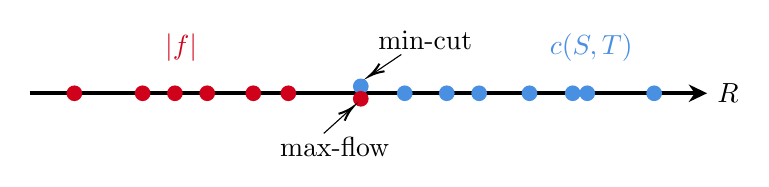
\begin{tikzpicture}[x=0.5pt,y=0.5pt,yscale=-1,xscale=1]
%uncomment if require: \path (0,126); %set diagram left start at 0, and has height of 126

%Straight Lines [id:da6845720994983642] 
\draw [line width=1.5]    (7,59) -- (492.5,59) ;
\draw [shift={(496.5,59)}, rotate = 180] [fill={rgb, 255:red, 0; green, 0; blue, 0 }  ][line width=0.08]  [draw opacity=0] (13.4,-6.43) -- (0,0) -- (13.4,6.44) -- (8.9,0) -- cycle    ;
%Shape: Circle [id:dp5839925944461984] 
\draw  [color={rgb, 255:red, 74; green, 144; blue, 226 }  ,draw opacity=1 ][fill={rgb, 255:red, 74; green, 144; blue, 226 }  ,fill opacity=1 ] (241,54) .. controls (241,51.1) and (243.35,48.75) .. (246.25,48.75) .. controls (249.15,48.75) and (251.5,51.1) .. (251.5,54) .. controls (251.5,56.9) and (249.15,59.25) .. (246.25,59.25) .. controls (243.35,59.25) and (241,56.9) .. (241,54) -- cycle ;
%Shape: Circle [id:dp34886579289539754] 
\draw  [color={rgb, 255:red, 208; green, 2; blue, 27 }  ,draw opacity=1 ][fill={rgb, 255:red, 208; green, 2; blue, 27 }  ,fill opacity=1 ] (188.65,59) .. controls (188.65,56.1) and (191,53.75) .. (193.9,53.75) .. controls (196.8,53.75) and (199.15,56.1) .. (199.15,59) .. controls (199.15,61.9) and (196.8,64.25) .. (193.9,64.25) .. controls (191,64.25) and (188.65,61.9) .. (188.65,59) -- cycle ;
%Shape: Circle [id:dp4135235202894928] 
\draw  [color={rgb, 255:red, 208; green, 2; blue, 27 }  ,draw opacity=1 ][fill={rgb, 255:red, 208; green, 2; blue, 27 }  ,fill opacity=1 ] (34,59) .. controls (34,56.1) and (36.35,53.75) .. (39.25,53.75) .. controls (42.15,53.75) and (44.5,56.1) .. (44.5,59) .. controls (44.5,61.9) and (42.15,64.25) .. (39.25,64.25) .. controls (36.35,64.25) and (34,61.9) .. (34,59) -- cycle ;
%Shape: Circle [id:dp20365687038540725] 
\draw  [color={rgb, 255:red, 208; green, 2; blue, 27 }  ,draw opacity=1 ][fill={rgb, 255:red, 208; green, 2; blue, 27 }  ,fill opacity=1 ] (83.33,59) .. controls (83.33,56.1) and (85.68,53.75) .. (88.58,53.75) .. controls (91.48,53.75) and (93.83,56.1) .. (93.83,59) .. controls (93.83,61.9) and (91.48,64.25) .. (88.58,64.25) .. controls (85.68,64.25) and (83.33,61.9) .. (83.33,59) -- cycle ;
%Shape: Circle [id:dp001936474221955753] 
\draw  [color={rgb, 255:red, 208; green, 2; blue, 27 }  ,draw opacity=1 ][fill={rgb, 255:red, 208; green, 2; blue, 27 }  ,fill opacity=1 ] (106.66,59) .. controls (106.66,56.1) and (109.01,53.75) .. (111.91,53.75) .. controls (114.81,53.75) and (117.16,56.1) .. (117.16,59) .. controls (117.16,61.9) and (114.81,64.25) .. (111.91,64.25) .. controls (109.01,64.25) and (106.66,61.9) .. (106.66,59) -- cycle ;
%Shape: Circle [id:dp8083671983789567] 
\draw  [color={rgb, 255:red, 208; green, 2; blue, 27 }  ,draw opacity=1 ][fill={rgb, 255:red, 208; green, 2; blue, 27 }  ,fill opacity=1 ] (129.99,59) .. controls (129.99,56.1) and (132.34,53.75) .. (135.24,53.75) .. controls (138.14,53.75) and (140.49,56.1) .. (140.49,59) .. controls (140.49,61.9) and (138.14,64.25) .. (135.24,64.25) .. controls (132.34,64.25) and (129.99,61.9) .. (129.99,59) -- cycle ;
%Shape: Circle [id:dp9076802577362922] 
\draw  [color={rgb, 255:red, 208; green, 2; blue, 27 }  ,draw opacity=1 ][fill={rgb, 255:red, 208; green, 2; blue, 27 }  ,fill opacity=1 ] (163.32,59) .. controls (163.32,56.1) and (165.67,53.75) .. (168.57,53.75) .. controls (171.47,53.75) and (173.82,56.1) .. (173.82,59) .. controls (173.82,61.9) and (171.47,64.25) .. (168.57,64.25) .. controls (165.67,64.25) and (163.32,61.9) .. (163.32,59) -- cycle ;
%Shape: Circle [id:dp4236178447115101] 
\draw  [color={rgb, 255:red, 208; green, 2; blue, 27 }  ,draw opacity=1 ][fill={rgb, 255:red, 208; green, 2; blue, 27 }  ,fill opacity=1 ] (241,63) .. controls (241,60.1) and (243.35,57.75) .. (246.25,57.75) .. controls (249.15,57.75) and (251.5,60.1) .. (251.5,63) .. controls (251.5,65.9) and (249.15,68.25) .. (246.25,68.25) .. controls (243.35,68.25) and (241,65.9) .. (241,63) -- cycle ;
%Shape: Circle [id:dp5050758022328539] 
\draw  [color={rgb, 255:red, 74; green, 144; blue, 226 }  ,draw opacity=1 ][fill={rgb, 255:red, 74; green, 144; blue, 226 }  ,fill opacity=1 ] (272.76,59) .. controls (272.76,56.1) and (275.11,53.75) .. (278.01,53.75) .. controls (280.91,53.75) and (283.26,56.1) .. (283.26,59) .. controls (283.26,61.9) and (280.91,64.25) .. (278.01,64.25) .. controls (275.11,64.25) and (272.76,61.9) .. (272.76,59) -- cycle ;
%Shape: Circle [id:dp8576227272464049] 
\draw  [color={rgb, 255:red, 74; green, 144; blue, 226 }  ,draw opacity=1 ][fill={rgb, 255:red, 74; green, 144; blue, 226 }  ,fill opacity=1 ] (303.14,59) .. controls (303.14,56.1) and (305.49,53.75) .. (308.39,53.75) .. controls (311.29,53.75) and (313.64,56.1) .. (313.64,59) .. controls (313.64,61.9) and (311.29,64.25) .. (308.39,64.25) .. controls (305.49,64.25) and (303.14,61.9) .. (303.14,59) -- cycle ;
%Shape: Circle [id:dp40578843932984965] 
\draw  [color={rgb, 255:red, 74; green, 144; blue, 226 }  ,draw opacity=1 ][fill={rgb, 255:red, 74; green, 144; blue, 226 }  ,fill opacity=1 ] (326.52,59) .. controls (326.52,56.1) and (328.87,53.75) .. (331.77,53.75) .. controls (334.67,53.75) and (337.02,56.1) .. (337.02,59) .. controls (337.02,61.9) and (334.67,64.25) .. (331.77,64.25) .. controls (328.87,64.25) and (326.52,61.9) .. (326.52,59) -- cycle ;
%Shape: Circle [id:dp2060326184335437] 
\draw  [color={rgb, 255:red, 74; green, 144; blue, 226 }  ,draw opacity=1 ][fill={rgb, 255:red, 74; green, 144; blue, 226 }  ,fill opacity=1 ] (362.9,59) .. controls (362.9,56.1) and (365.25,53.75) .. (368.15,53.75) .. controls (371.05,53.75) and (373.4,56.1) .. (373.4,59) .. controls (373.4,61.9) and (371.05,64.25) .. (368.15,64.25) .. controls (365.25,64.25) and (362.9,61.9) .. (362.9,59) -- cycle ;
%Shape: Circle [id:dp7156703955132185] 
\draw  [color={rgb, 255:red, 74; green, 144; blue, 226 }  ,draw opacity=1 ][fill={rgb, 255:red, 74; green, 144; blue, 226 }  ,fill opacity=1 ] (394.16,59) .. controls (394.16,56.1) and (396.51,53.75) .. (399.41,53.75) .. controls (402.31,53.75) and (404.66,56.1) .. (404.66,59) .. controls (404.66,61.9) and (402.31,64.25) .. (399.41,64.25) .. controls (396.51,64.25) and (394.16,61.9) .. (394.16,59) -- cycle ;
%Shape: Circle [id:dp5714468634699819] 
\draw  [color={rgb, 255:red, 74; green, 144; blue, 226 }  ,draw opacity=1 ][fill={rgb, 255:red, 74; green, 144; blue, 226 }  ,fill opacity=1 ] (404.66,59) .. controls (404.66,56.1) and (407.01,53.75) .. (409.91,53.75) .. controls (412.81,53.75) and (415.16,56.1) .. (415.16,59) .. controls (415.16,61.9) and (412.81,64.25) .. (409.91,64.25) .. controls (407.01,64.25) and (404.66,61.9) .. (404.66,59) -- cycle ;
%Shape: Circle [id:dp338221725625915] 
\draw  [color={rgb, 255:red, 74; green, 144; blue, 226 }  ,draw opacity=1 ][fill={rgb, 255:red, 74; green, 144; blue, 226 }  ,fill opacity=1 ] (453,59) .. controls (453,56.1) and (455.35,53.75) .. (458.25,53.75) .. controls (461.15,53.75) and (463.5,56.1) .. (463.5,59) .. controls (463.5,61.9) and (461.15,64.25) .. (458.25,64.25) .. controls (455.35,64.25) and (453,61.9) .. (453,59) -- cycle ;
%Straight Lines [id:da046923477941067104] 
\draw    (219.5,88) -- (239.02,70.34) ;
\draw [shift={(240.5,69)}, rotate = 497.86] [color={rgb, 255:red, 0; green, 0; blue, 0 }  ][line width=0.75]    (10.93,-3.29) .. controls (6.95,-1.4) and (3.31,-0.3) .. (0,0) .. controls (3.31,0.3) and (6.95,1.4) .. (10.93,3.29)   ;
%Straight Lines [id:da008869050799750533] 
\draw    (275.5,31) -- (254.16,45.38) ;
\draw [shift={(252.5,46.5)}, rotate = 326.02] [color={rgb, 255:red, 0; green, 0; blue, 0 }  ][line width=0.75]    (10.93,-3.29) .. controls (6.95,-1.4) and (3.31,-0.3) .. (0,0) .. controls (3.31,0.3) and (6.95,1.4) .. (10.93,3.29)   ;

% Text Node
\draw (502,50) node [anchor=north west][inner sep=0.75pt]   [align=left] {$\displaystyle R$};
% Text Node
\draw (103,14) node [anchor=north west][inner sep=0.75pt]   [align=left] {$\displaystyle \textcolor[rgb]{0.82,0.01,0.11}{| f| }$};
% Text Node
\draw (381,14) node [anchor=north west][inner sep=0.75pt]   [align=left] {$\displaystyle \textcolor[rgb]{0.29,0.56,0.89}{c( S,T)}$};
% Text Node
\draw (186,89) node [anchor=north west][inner sep=0.75pt]   [align=left] {\textcolor[rgb]{0,0,0}{max-flow}};
% Text Node
\draw (257,12) node [anchor=north west][inner sep=0.75pt]   [align=left] {\textcolor[rgb]{0,0,0}{min-cut}};


\end{tikzpicture}

}
\caption{Illustration of the relationship between capacity of any $s$-$t$ cut
and value of \emph{any} $s$-$t$ flow.}
\label{fig:flow-meet}
\end{figure}

Claim~\ref{claim1} states that capacity of \emph{any} $s$-$t$ cut
is larger or equal to the value of \emph{any} $s$-$t$ flow.
Consequently, if there exists an $s$-$t$ flow $f$ and an $s$-$t$ cut $(S,T)$
satisfies that $|f| = c(S, T)$, then this $f$ must be a maximum-flow,
and this $(S, T)$ must be a minimum-cut.
An illustration of this property is given in Figure~\ref{fig:flow-meet},
where each red point represents the value of an $s$-$t$ flow
while each blue point represents the capacity of an $s$-$t$ cut.
So all red points lie to the left side of all blue points,
and if a red point and a blue point meet, they are maximum-flow and minimum-cut.


\begin{figure}[h]
\centering{

\tikzset{every picture/.style={line width=0.75pt}} %set default line width to 0.75pt        

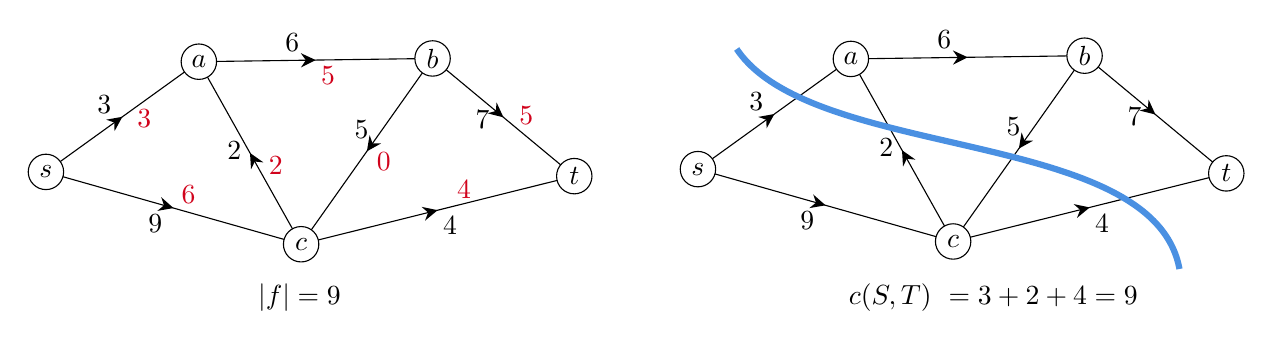
\begin{tikzpicture}[x=0.5pt,y=0.5pt,yscale=-1,xscale=1]
%uncomment if require: \path (0,225); %set diagram left start at 0, and has height of 225

%Straight Lines [id:da9082688563234774] 
\draw    (236.22,169.11) -- (331.22,34.84) ;
\draw [shift={(283.72,101.98)}, rotate = 305.28] [fill={rgb, 255:red, 0; green, 0; blue, 0 }  ][line width=0.08]  [draw opacity=0] (10.72,-5.15) -- (0,0) -- (10.72,5.15) -- (7.12,0) -- cycle    ;
%Straight Lines [id:da4024226568643945] 
\draw    (162.31,37.18) -- (236.22,169.11) ;
\draw [shift={(199.27,103.14)}, rotate = 60.74] [fill={rgb, 255:red, 0; green, 0; blue, 0 }  ][line width=0.08]  [draw opacity=0] (10.72,-5.15) -- (0,0) -- (10.72,5.15) -- (7.12,0) -- cycle    ;
%Straight Lines [id:da7912195585462996] 
\draw    (51.79,116.83) -- (236.22,169.11) ;
\draw [shift={(144.01,142.97)}, rotate = 195.83] [fill={rgb, 255:red, 0; green, 0; blue, 0 }  ][line width=0.08]  [draw opacity=0] (10.72,-5.15) -- (0,0) -- (10.72,5.15) -- (7.12,0) -- cycle    ;
%Straight Lines [id:da213272602991051] 
\draw    (433.62,119.9) -- (236.22,169.11) ;
\draw [shift={(334.92,144.5)}, rotate = 166] [fill={rgb, 255:red, 0; green, 0; blue, 0 }  ][line width=0.08]  [draw opacity=0] (10.72,-5.15) -- (0,0) -- (10.72,5.15) -- (7.12,0) -- cycle    ;
%Straight Lines [id:da8511890231681417] 
\draw    (51.79,116.83) -- (162.31,37.18) ;
\draw [shift={(107.05,77)}, rotate = 144.22] [fill={rgb, 255:red, 0; green, 0; blue, 0 }  ][line width=0.08]  [draw opacity=0] (10.72,-5.15) -- (0,0) -- (10.72,5.15) -- (7.12,0) -- cycle    ;
%Straight Lines [id:da36886265290248843] 
\draw    (331.22,34.84) -- (433.62,119.9) ;
\draw [shift={(382.42,77.37)}, rotate = 219.71] [fill={rgb, 255:red, 0; green, 0; blue, 0 }  ][line width=0.08]  [draw opacity=0] (10.72,-5.15) -- (0,0) -- (10.72,5.15) -- (7.12,0) -- cycle    ;
%Straight Lines [id:da5107251195982034] 
\draw    (162.31,37.18) -- (331.22,34.84) ;
\draw [shift={(246.76,36.01)}, rotate = 179.21] [fill={rgb, 255:red, 0; green, 0; blue, 0 }  ][line width=0.08]  [draw opacity=0] (10.72,-5.15) -- (0,0) -- (10.72,5.15) -- (7.12,0) -- cycle    ;
%Shape: Ellipse [id:dp4938989418762101] 
\draw  [fill={rgb, 255:red, 255; green, 255; blue, 255 }  ,fill opacity=1 ] (39,116.83) .. controls (39,109.77) and (44.73,104.04) .. (51.79,104.04) .. controls (58.86,104.04) and (64.58,109.77) .. (64.58,116.83) .. controls (64.58,123.9) and (58.86,129.62) .. (51.79,129.62) .. controls (44.73,129.62) and (39,123.9) .. (39,116.83) -- cycle ;
%Shape: Ellipse [id:dp7740460741911303] 
\draw  [fill={rgb, 255:red, 255; green, 255; blue, 255 }  ,fill opacity=1 ] (149.52,37.18) .. controls (149.52,30.11) and (155.25,24.39) .. (162.31,24.39) .. controls (169.38,24.39) and (175.1,30.11) .. (175.1,37.18) .. controls (175.1,44.24) and (169.38,49.97) .. (162.31,49.97) .. controls (155.25,49.97) and (149.52,44.24) .. (149.52,37.18) -- cycle ;
%Shape: Ellipse [id:dp7874695049462108] 
\draw  [fill={rgb, 255:red, 255; green, 255; blue, 255 }  ,fill opacity=1 ] (318.43,34.84) .. controls (318.43,27.78) and (324.15,22.05) .. (331.22,22.05) .. controls (338.28,22.05) and (344.01,27.78) .. (344.01,34.84) .. controls (344.01,41.9) and (338.28,47.63) .. (331.22,47.63) .. controls (324.15,47.63) and (318.43,41.9) .. (318.43,34.84) -- cycle ;
%Shape: Ellipse [id:dp5976477726175576] 
\draw  [fill={rgb, 255:red, 255; green, 255; blue, 255 }  ,fill opacity=1 ] (223.43,169.11) .. controls (223.43,162.05) and (229.15,156.32) .. (236.22,156.32) .. controls (243.28,156.32) and (249.01,162.05) .. (249.01,169.11) .. controls (249.01,176.18) and (243.28,181.9) .. (236.22,181.9) .. controls (229.15,181.9) and (223.43,176.18) .. (223.43,169.11) -- cycle ;
%Shape: Ellipse [id:dp8582649844509285] 
\draw  [fill={rgb, 255:red, 255; green, 255; blue, 255 }  ,fill opacity=1 ] (420.83,119.9) .. controls (420.83,112.83) and (426.56,107.11) .. (433.62,107.11) .. controls (440.69,107.11) and (446.41,112.83) .. (446.41,119.9) .. controls (446.41,126.96) and (440.69,132.69) .. (433.62,132.69) .. controls (426.56,132.69) and (420.83,126.96) .. (420.83,119.9) -- cycle ;
%Straight Lines [id:da7220126124754225] 
\draw    (707.43,167.11) -- (802.42,32.84) ;
\draw [shift={(754.92,99.98)}, rotate = 305.28] [fill={rgb, 255:red, 0; green, 0; blue, 0 }  ][line width=0.08]  [draw opacity=0] (10.72,-5.15) -- (0,0) -- (10.72,5.15) -- (7.12,0) -- cycle    ;
%Straight Lines [id:da8450888320434884] 
\draw    (633.52,35.18) -- (707.43,167.11) ;
\draw [shift={(670.47,101.14)}, rotate = 60.74] [fill={rgb, 255:red, 0; green, 0; blue, 0 }  ][line width=0.08]  [draw opacity=0] (10.72,-5.15) -- (0,0) -- (10.72,5.15) -- (7.12,0) -- cycle    ;
%Straight Lines [id:da28397437899635924] 
\draw    (523,114.83) -- (707.43,167.11) ;
\draw [shift={(615.21,140.97)}, rotate = 195.83] [fill={rgb, 255:red, 0; green, 0; blue, 0 }  ][line width=0.08]  [draw opacity=0] (10.72,-5.15) -- (0,0) -- (10.72,5.15) -- (7.12,0) -- cycle    ;
%Straight Lines [id:da37734529713635245] 
\draw    (904.83,117.9) -- (707.43,167.11) ;
\draw [shift={(806.13,142.5)}, rotate = 166] [fill={rgb, 255:red, 0; green, 0; blue, 0 }  ][line width=0.08]  [draw opacity=0] (10.72,-5.15) -- (0,0) -- (10.72,5.15) -- (7.12,0) -- cycle    ;
%Straight Lines [id:da0928727354789407] 
\draw    (523,114.83) -- (633.52,35.18) ;
\draw [shift={(578.26,75)}, rotate = 144.22] [fill={rgb, 255:red, 0; green, 0; blue, 0 }  ][line width=0.08]  [draw opacity=0] (10.72,-5.15) -- (0,0) -- (10.72,5.15) -- (7.12,0) -- cycle    ;
%Straight Lines [id:da48901200769836506] 
\draw    (802.42,32.84) -- (904.83,117.9) ;
\draw [shift={(853.63,75.37)}, rotate = 219.71] [fill={rgb, 255:red, 0; green, 0; blue, 0 }  ][line width=0.08]  [draw opacity=0] (10.72,-5.15) -- (0,0) -- (10.72,5.15) -- (7.12,0) -- cycle    ;
%Straight Lines [id:da42638454833244943] 
\draw    (633.52,35.18) -- (802.42,32.84) ;
\draw [shift={(717.97,34.01)}, rotate = 179.21] [fill={rgb, 255:red, 0; green, 0; blue, 0 }  ][line width=0.08]  [draw opacity=0] (10.72,-5.15) -- (0,0) -- (10.72,5.15) -- (7.12,0) -- cycle    ;
%Shape: Ellipse [id:dp8396933555638321] 
\draw  [fill={rgb, 255:red, 255; green, 255; blue, 255 }  ,fill opacity=1 ] (510.21,114.83) .. controls (510.21,107.77) and (515.94,102.04) .. (523,102.04) .. controls (530.06,102.04) and (535.79,107.77) .. (535.79,114.83) .. controls (535.79,121.9) and (530.06,127.62) .. (523,127.62) .. controls (515.94,127.62) and (510.21,121.9) .. (510.21,114.83) -- cycle ;
%Shape: Ellipse [id:dp26514516487162165] 
\draw  [fill={rgb, 255:red, 255; green, 255; blue, 255 }  ,fill opacity=1 ] (620.73,35.18) .. controls (620.73,28.11) and (626.46,22.39) .. (633.52,22.39) .. controls (640.58,22.39) and (646.31,28.11) .. (646.31,35.18) .. controls (646.31,42.24) and (640.58,47.97) .. (633.52,47.97) .. controls (626.46,47.97) and (620.73,42.24) .. (620.73,35.18) -- cycle ;
%Shape: Ellipse [id:dp08880583589515356] 
\draw  [fill={rgb, 255:red, 255; green, 255; blue, 255 }  ,fill opacity=1 ] (789.63,32.84) .. controls (789.63,25.78) and (795.36,20.05) .. (802.42,20.05) .. controls (809.49,20.05) and (815.21,25.78) .. (815.21,32.84) .. controls (815.21,39.9) and (809.49,45.63) .. (802.42,45.63) .. controls (795.36,45.63) and (789.63,39.9) .. (789.63,32.84) -- cycle ;
%Shape: Ellipse [id:dp5357688919708571] 
\draw  [fill={rgb, 255:red, 255; green, 255; blue, 255 }  ,fill opacity=1 ] (694.64,167.11) .. controls (694.64,160.05) and (700.36,154.32) .. (707.43,154.32) .. controls (714.49,154.32) and (720.22,160.05) .. (720.22,167.11) .. controls (720.22,174.18) and (714.49,179.9) .. (707.43,179.9) .. controls (700.36,179.9) and (694.64,174.18) .. (694.64,167.11) -- cycle ;
%Shape: Ellipse [id:dp8198953137865064] 
\draw  [fill={rgb, 255:red, 255; green, 255; blue, 255 }  ,fill opacity=1 ] (892.04,117.9) .. controls (892.04,110.83) and (897.77,105.11) .. (904.83,105.11) .. controls (911.89,105.11) and (917.62,110.83) .. (917.62,117.9) .. controls (917.62,124.96) and (911.89,130.69) .. (904.83,130.69) .. controls (897.77,130.69) and (892.04,124.96) .. (892.04,117.9) -- cycle ;
%Curve Lines [id:da631287332539116] 
\draw [color={rgb, 255:red, 74; green, 144; blue, 226 }  ,draw opacity=1 ][line width=2.25]    (551,28) .. controls (606,110) and (852,84) .. (871,187) ;

% Text Node
\draw (51.79,116.83) node   [align=left] {$\displaystyle s$};
% Text Node
\draw (162.31,37.18) node   [align=left] {$\displaystyle a$};
% Text Node
\draw (331.22,34.84) node   [align=left] {$\displaystyle b$};
% Text Node
\draw (236.22,169.11) node   [align=left] {$\displaystyle c$};
% Text Node
\draw (433.62,119.9) node   [align=left] {$\displaystyle t$};
% Text Node
\draw (124,146) node [anchor=north west][inner sep=0.75pt]   [align=left] {$\displaystyle 9$};
% Text Node
\draw (273,78) node [anchor=north west][inner sep=0.75pt]   [align=left] {$\displaystyle 5$};
% Text Node
\draw (181,93) node [anchor=north west][inner sep=0.75pt]   [align=left] {$\displaystyle 2$};
% Text Node
\draw (87,60) node [anchor=north west][inner sep=0.75pt]   [align=left] {$\displaystyle 3$};
% Text Node
\draw (336.92,147.5) node [anchor=north west][inner sep=0.75pt]   [align=left] {$\displaystyle 4$};
% Text Node
\draw (360.42,70.37) node [anchor=north west][inner sep=0.75pt]   [align=left] {$\displaystyle 7$};
% Text Node
\draw (223,15) node [anchor=north west][inner sep=0.75pt]   [align=left] {$\displaystyle 6$};
% Text Node
\draw (148,125) node [anchor=north west][inner sep=0.75pt]   [align=left] {$\displaystyle \textcolor[rgb]{0.82,0.01,0.11}{6}$};
% Text Node
\draw (211,104) node [anchor=north west][inner sep=0.75pt]   [align=left] {$\displaystyle \textcolor[rgb]{0.82,0.01,0.11}{2}$};
% Text Node
\draw (347,121) node [anchor=north west][inner sep=0.75pt]   [align=left] {$\displaystyle \textcolor[rgb]{0.82,0.01,0.11}{4}$};
% Text Node
\draw (116,70) node [anchor=north west][inner sep=0.75pt]   [align=left] {$\displaystyle \textcolor[rgb]{0.82,0.01,0.11}{3}$};
% Text Node
\draw (248.76,39.01) node [anchor=north west][inner sep=0.75pt]   [align=left] {$\displaystyle \textcolor[rgb]{0.82,0.01,0.11}{5}$};
% Text Node
\draw (289,101) node [anchor=north west][inner sep=0.75pt]   [align=left] {$\displaystyle \textcolor[rgb]{0.82,0.01,0.11}{0}$};
% Text Node
\draw (392,68) node [anchor=north west][inner sep=0.75pt]   [align=left] {$\displaystyle \textcolor[rgb]{0.82,0.01,0.11}{5}$};
% Text Node
\draw (523,114.83) node   [align=left] {$\displaystyle s$};
% Text Node
\draw (633.52,35.18) node   [align=left] {$\displaystyle a$};
% Text Node
\draw (802.42,32.84) node   [align=left] {$\displaystyle b$};
% Text Node
\draw (707.43,167.11) node   [align=left] {$\displaystyle c$};
% Text Node
\draw (904.83,117.9) node   [align=left] {$\displaystyle t$};
% Text Node
\draw (595.21,144) node [anchor=north west][inner sep=0.75pt]   [align=left] {$\displaystyle 9$};
% Text Node
\draw (744.21,76) node [anchor=north west][inner sep=0.75pt]   [align=left] {$\displaystyle 5$};
% Text Node
\draw (652.21,91) node [anchor=north west][inner sep=0.75pt]   [align=left] {$\displaystyle 2$};
% Text Node
\draw (558.21,58) node [anchor=north west][inner sep=0.75pt]   [align=left] {$\displaystyle 3$};
% Text Node
\draw (808.13,145.5) node [anchor=north west][inner sep=0.75pt]   [align=left] {$\displaystyle 4$};
% Text Node
\draw (831.63,68.37) node [anchor=north west][inner sep=0.75pt]   [align=left] {$\displaystyle 7$};
% Text Node
\draw (694.21,13) node [anchor=north west][inner sep=0.75pt]   [align=left] {$\displaystyle 6$};
% Text Node
\draw (630.21,196) node [anchor=north west][inner sep=0.75pt]   [align=left] {$\displaystyle c( S,T) \ =3+2+4=9$};
% Text Node
\draw (203.21,196) node [anchor=north west][inner sep=0.75pt]   [align=left] {$\displaystyle |f|=9$};


\end{tikzpicture}

}
\caption{A maximum-flow $f$ and a minimum cut $(S, T)$, verified by $|f| = c(S,T)$.}
\label{fig:maxflow-mincut}
\end{figure}

In above example, we see a flow $f$ with $|f| = 9$ and an $s$-$t$ cut $(S, T)$ with $c(S, T) = 9$.
So both are optimal. See Figure~\ref{fig:maxflow-mincut}.

